\documentclass[10pt]{beamer}
\usetheme{metropolis}
% all imports
\usepackage[utf8]{inputenc}
\usepackage[T1]{fontenc}
\usepackage{lmodern}
\usepackage{appendixnumberbeamer}
\usepackage{hyperref}
\usepackage{booktabs}
\usepackage{bm}
\usepackage[scale=2]{ccicons}
\usepackage[outputdir=build]{minted}
\usepackage{pgfplots}
\usepackage{array,colortbl,xcolor}
\usepgfplotslibrary{dateplot}
\usepackage{setspace}
\usepackage{etoolbox}
\usepackage{xspace}
\usepackage{tikz}
\usetikzlibrary{shapes,arrows,positioning,fit,backgrounds}
\usepackage{tkz-euclide}

\AtBeginEnvironment{quote}{\singlespacing}

\AtBeginEnvironment{quote}{\singlespacing}

% new commands
\newcommand{\themename}{\textbf{\textsc{metropolis}}\xspace}
\newcommand{\vect}[1]{\bm{#1}}
\newcommand{\myprime}[1]{{#1}^{\prime}}
\newcommand{\grad}[2]{\nabla_{#1} {#2}}
\newcommand{\dotp}[2]{{#1}^{\top}{#2}}
\newcommand{\dotpPright}[2]{{#1}^{\top}\left({#2}\right)}
\newcommand{\outerp}[2]{\left({#1}\right){#2}^{\top}}
\newcommand{\Jacobian}[2]{\frac{\partial #1}{\partial #2}}
\newcommand{\Vocab}{\mathbb{V}}

% definitions
\definecolor{blue}{RGB}{159, 192, 176}
\definecolor{green}{RGB}{160, 227, 127}
\definecolor{orange}{RGB}{243, 188, 125}
\definecolor{red}{RGB}{253, 123, 84}
\definecolor{nephritis}{RGB}{39, 174, 96}
\definecolor{emerald}{RGB}{46, 204, 113}
\definecolor{turquoise}{RGB}{39, 174, 96}
\definecolor{green-sea}{RGB}{22, 160, 133}
% Tikzstyles for Computation Graphs

% nodes
\tikzstyle{noop} = [circle, draw=none, fill=red, minimum size = 10pt]
\tikzstyle{op} = [circle, draw=red, line width=1.5pt, fill=red!70, text=black, text centered, font=\bf \normalsize, minimum size = 25pt]
\tikzstyle{state} = [circle, draw=blue, line width=1.5pt, fill=blue!70, text=black, text centered, font=\bf \normalsize, minimum size = 25pt]
% \tikzstyle{gradient} = [circle, draw=green, line width=1.5pt, fill=green!60, text=black, text centered, font=\bf \normalsize, minimum size = 25pt]
\tikzstyle{gradient} = [circle, draw=nephritis, line width=1.5pt, fill=nephritis!60, text=black, text centered, font=\bf \normalsize, minimum size = 25pt]
\tikzstyle{textonly} = [draw=none, fill=none, text centered, font=\bf \normalsize]

% edges
% \tikzstyle{tedge}  = [draw, thick, >=stealth, ->]
\tikzstyle{tedge}  = [draw, thick, >=latex, ->]

% namedscope
\tikzstyle{namedscope} = [circle, draw=orange, line width=1.5pt, fill=orange!60, align=center, inner sep=0pt]

% \tikzstyle{container} = [draw=none, rectangle, dotted, inner ysep=1.5em]
% \tikzstyle{novertex} = [draw=none, fill=none, text centered]
% \tikzstyle{predicate} = [ellipse, draw, thick, text centered, rounded corners, minimum size=30pt]
% \tikzstyle{aux} = [rectangle, draw, thick, text centered, rounded corners, minimum size=30pt]
% \tikzstyle{ledge}  = [draw, dashed, thick, >=stealth, ->]
% \tikzstyle{pedge}  = [draw, thick, >=stealth, ->]



\title{An introduction to Recurrent Neural Networks}
\date{\today}

\author{
  Felipe Salvatore\\
  \url{https://felipessalvatore.github.io/}
  \vspace{0.4 cm}
  \and\\ 
  Thiago Bueno\\
  \url{http://thiagopbueno.github.io/}\\\vspace{0.4 cm}
}

\institute{\textbf{IME-USP}: Institute of Mathematics and Statistics from the University of São Paulo}


\begin{document}

\maketitle

\section{Introduction}

\begin{frame}[fragile]{Basic idea}
\begin{itemize}
\item A \alert{Recurrent Neural Network (RNN)} allows us to operate over \textbf{sequences} of vectors: either sequences in the \textbf{input} or the \textbf{output} 
\vspace{0.5cm}
\item This feature differentiate the RNN model from other deep learning architectures such as \textbf{Deep Feedforward Network (DFN)} and \textbf{Convolutional Neural Network (CNN)}.
\end{itemize}
\end{frame}

\begin{frame}[fragile]{DFN and CNN}
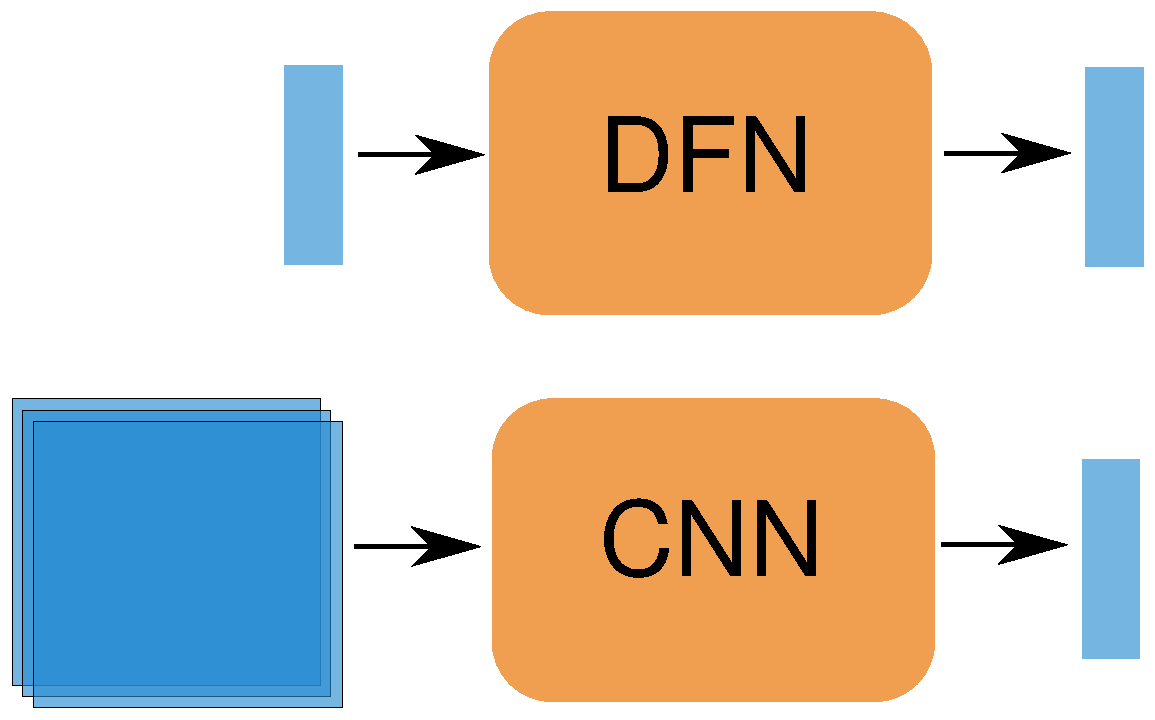
\includegraphics[scale=0.5]{images/DfnCnn.pdf}
\end{frame}

\begin{frame}[fragile]{RNN: unfold representation}
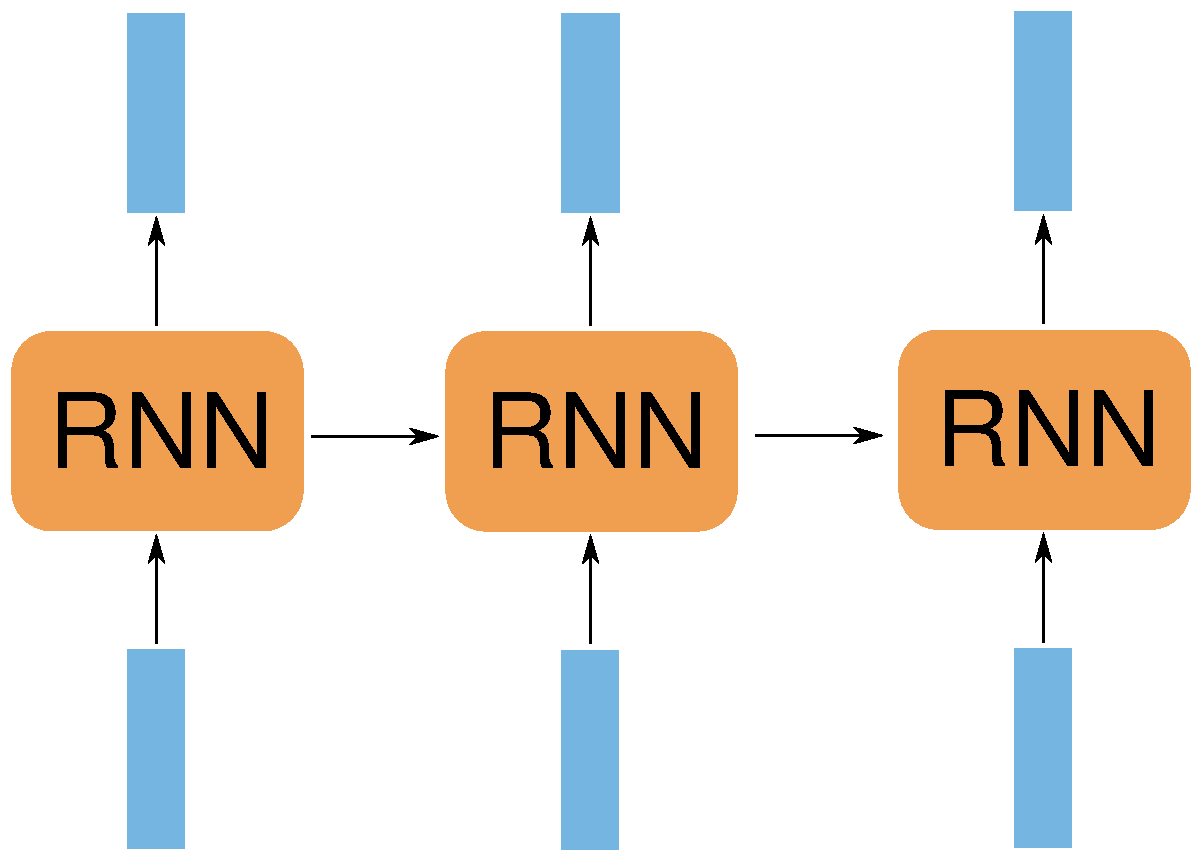
\includegraphics[scale=0.5]{images/RNNnaive1.pdf}
\end{frame}

\begin{frame}[fragile]{RNN: cyclic representation}
\begin{center}
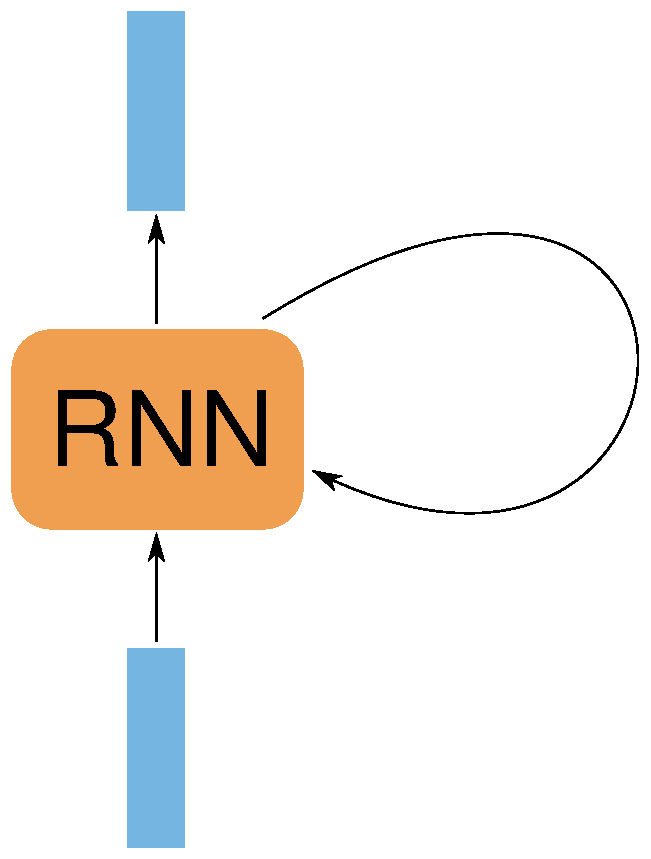
\includegraphics[scale=0.5]{images/RNNnaive2.pdf}
\end{center}
\end{frame}


\section{Graph Representation}

\begin{frame}[fragile]{NN as a directed graph: old version}
\begin{figure}[ht!]
\centering

\scalebox{1.2}{
\begin{tikzpicture}[auto]

% operations =============================
\node[op] (x2) {$x_2$};
\node[op, above=40pt of x2] (x1) {$x_1$};
\node[op, below=40pt of x2] (x3) {$x_3$};
\node[op, right=60pt of x2] (vk) {$v_k$};
\node[op, right=40pt of vk] (yk) {$y_k$};
\node[textonly, below right=20pt of x3] (Synaptic) {Synaptic link};
\node[textonly, below right=50pt of vk] (Activation) {Activation link};


% edges
\path[tedge] (x1) edge node[above=1.8pt] {$\vect{W}_{k,1}$} (vk);
\path[tedge] (x2) edge node[above=0.2pt] {$\vect{W}_{k,2}$} (vk);
\path[tedge] (x3) edge node[above=3.8pt] {$\vect{W}_{k,3}$} (vk);
\path[tedge] (vk) edge node[above=1pt] {{\Large$f$}}  (yk) ;

% info edges
\draw[orange!120, line width=1mm]  (Synaptic) to [out=150,in=0] (x3);
\draw[orange!120, line width=1mm] (Synaptic) to [out=150,in=-100] (vk);

\draw[orange!120, line width=1mm]  (Activation) to [out=170,in=-40] (vk);
\draw[orange!120, line width=1mm] (Activation) to [out=170,in=-100] (yk);



\end{tikzpicture}
} % scalebox
\end{figure}

\end{frame}

\begin{frame}[fragile]{NN as a directed graph: old version}
\begin{figure}[ht!]
\centering

\scalebox{0.7}{
\begin{tikzpicture}[auto]

% operations =============================

% input layer
\node[op] (x5) {$x_5$};
\node[op, above=2.5pt of x5] (x4) {$x_4$};
\node[op, above=2.5pt of x4] (x3) {$x_3$};
\node[op, above=2.5pt of x3] (x2) {$x_2$};
\node[op, above=2.5pt of x2] (x1) {$x_1$};
\node[op, below=2.5pt of x5] (x6) {$x_6$};
\node[op, below=2.5pt of x6] (x7) {$x_7$};
\node[op, below=2.5pt of x7] (x8) {$x_8$};
\node[op, below=2.5pt of x8] (x9) {$x_9$};
\node[op, below=2.5pt of x9] (x10) {$x_{10}$};

% hidden layer
\node[op,  right=130pt of x5] (v2) {$v_2$};
\node[op, below=2.5pt of v2] (v3) {$v_3$};
\node[op, below=2.5pt of v3] (v4) {$v_4$};
\node[op, above=2.5pt of v2] (v1) {$v_1$};

\node[op,  right=40pt of v2] (h2) {$h_2$};
\node[op, below=2.5pt of h2] (h3) {$h_3$};
\node[op, below=2.5pt of h3] (h4) {$h_4$};
\node[op, above=2.5pt of h2] (h1) {$h_1$};


% output layer
\node[op,  right=60pt of h2] (z1) {$z_1$};
\node[op,  right=60pt of h3] (z2) {$z_2$};

\node[op,  right=50pt of z1] (y1) {$\hat{y}_1$};
\node[op,  right=50pt of z2] (y2) {$\hat{y}_2$};


% edges input layer to hidden
\path[tedge] (x1) -- (v1);
\path[tedge] (x1) -- (v2);
\path[tedge] (x1) -- (v3);
\path[tedge] (x1) -- (v4);

\path[tedge] (x2) -- (v1);
\path[tedge] (x2) -- (v2);
\path[tedge] (x2) -- (v3);
\path[tedge] (x2) -- (v4);

\path[tedge] (x3) -- (v1);
\path[tedge] (x3) -- (v2);
\path[tedge] (x3) -- (v3);
\path[tedge] (x3) -- (v4);

\path[tedge] (x4) -- (v1);
\path[tedge] (x4) -- (v2);
\path[tedge] (x4) -- (v3);
\path[tedge] (x4) -- (v4);

\path[tedge] (x5) -- (v1);
\path[tedge] (x5) -- (v2);
\path[tedge] (x5) -- (v3);
\path[tedge] (x5) -- (v4);

\path[tedge] (x6) -- (v1);
\path[tedge] (x6) -- (v2);
\path[tedge] (x6) -- (v3);
\path[tedge] (x6) -- (v4);

\path[tedge] (x7) -- (v1);
\path[tedge] (x7) -- (v2);
\path[tedge] (x7) -- (v3);
\path[tedge] (x7) -- (v4);

\path[tedge] (x8) -- (v1);
\path[tedge] (x8) -- (v2);
\path[tedge] (x8) -- (v3);
\path[tedge] (x8) -- (v4);

\path[tedge] (x9) -- (v1);
\path[tedge] (x9) -- (v2);
\path[tedge] (x9) -- (v3);
\path[tedge] (x9) -- (v4);

\path[tedge] (x10) -- (v1);
\path[tedge] (x10) -- (v2);
\path[tedge] (x10) -- (v3);
\path[tedge] (x10) -- (v4);

% edges hidden to hidden
\path[tedge] (v1) edge node[above=1pt] {{\Large$\sigma$}}  (h1) ;
\path[tedge] (v2) edge node[above=1pt] {{\Large$\sigma$}}  (h2) ;
\path[tedge] (v3) edge node[above=1pt] {{\Large$\sigma$}}  (h3) ;
\path[tedge] (v4) edge node[above=1pt] {{\Large$\sigma$}}  (h4) ;

% edges hidden to output
\path[tedge] (h1) -- (z1);
\path[tedge] (h1) -- (z2);

\path[tedge] (h2) -- (z1);
\path[tedge] (h2) -- (z2);

\path[tedge] (h3) -- (z1);
\path[tedge] (h3) -- (z2);

\path[tedge] (h4) -- (z1);
\path[tedge] (h4) -- (z2);

% edges output to output
\path[tedge] (z1) edge node[above=1pt] {{\Large softmax}}  (y1) ;
\path[tedge] (z2) edge node[above=1pt] {{\Large softmax}}  (y2) ;




\end{tikzpicture}
} % scalebox
\end{figure}

\end{frame}

\begin{frame}{Recap: basic functions}
\Large{
 \vspace{0.2cm}
\begin{equation*}
\sigma(x) = \frac{1}{1 + e^{-x}}
\end{equation*}
\vspace{0.5cm}
 \begin{equation*}
softmax(x) = \frac{e^{x}}{\sum e^{x}}
\end{equation*}
}
\end{frame}



\begin{frame}[fragile]{NN as a directed graph: old version}
\begin{figure}[ht!]
\centering

\scalebox{0.7}{
\begin{tikzpicture}[auto]

% operations =============================

% input layer
\node[op] (x5) {};
\node[op, above=2.5pt of x5] (x4) {};
\node[op, above=2.5pt of x4] (x3) {};
\node[op, above=2.5pt of x3] (x2) {};
\node[op, above=2.5pt of x2] (x1) {};
\node[op, below=2.5pt of x5] (x6) {};
\node[op, below=2.5pt of x6] (x7) {};
\node[op, below=2.5pt of x7] (x8) {};
\node[op, below=2.5pt of x8] (x9) {};
\node[op, below=2.5pt of x9] (x10) {};

\node[textonly, above=2.5pt of x1] (x) {{\LARGE$\vect{x}$}};
\node[textonly, below=4.5pt of x10] (input) {{\large Input layer}};

% hidden layer
\node[op,  right=130pt of x5] (h2) {};
\node[op, below=2.5pt of h2] (h3) {};
\node[op, below=2.5pt of h3] (h4) {};
\node[op, above=2.5pt of h2] (h1) {};

\node[textonly, above=2.5pt of h1] (h) {{\LARGE$\vect{h}$}};
\node[textonly, below=4.5pt of h4] (hidden) {{\large Hidden layer}};

% output layer
\node[op,  right=60pt of h2] (y1) {};
\node[op,  right=60pt of h3] (y2) {};

\node[textonly, above=2.5pt of y1] (y) {{\LARGE$\hat{\vect{y}}$}};
\node[textonly, below=4.5pt of y2] (output) {{\large Output layer}};

% edges input layer to hidden
\path[tedge] (x1) -- (h1);
\path[tedge] (x1) -- (h2);
\path[tedge] (x1) -- (h3);
\path[tedge] (x1) -- (h4);

\path[tedge] (x2) -- (h1);
\path[tedge] (x2) -- (h2);
\path[tedge] (x2) -- (h3);
\path[tedge] (x2) -- (h4);

\path[tedge] (x3) -- (h1);
\path[tedge] (x3) -- (h2);
\path[tedge] (x3) -- (h3);
\path[tedge] (x3) -- (h4);

\path[tedge] (x4) -- (h1);
\path[tedge] (x4) -- (h2);
\path[tedge] (x4) -- (h3);
\path[tedge] (x4) -- (h4);

\path[tedge] (x5) -- (h1);
\path[tedge] (x5) -- (h2);
\path[tedge] (x5) -- (h3);
\path[tedge] (x5) -- (h4);

\path[tedge] (x6) -- (h1);
\path[tedge] (x6) -- (h2);
\path[tedge] (x6) -- (h3);
\path[tedge] (x6) -- (h4);

\path[tedge] (x7) -- (h1);
\path[tedge] (x7) -- (h2);
\path[tedge] (x7) -- (h3);
\path[tedge] (x7) -- (h4);

\path[tedge] (x8) -- (h1);
\path[tedge] (x8) -- (h2);
\path[tedge] (x8) -- (h3);
\path[tedge] (x8) -- (h4);

\path[tedge] (x9) -- (h1);
\path[tedge] (x9) -- (h2);
\path[tedge] (x9) -- (h3);
\path[tedge] (x9) -- (h4);

\path[tedge] (x10) -- (h1);
\path[tedge] (x10) -- (h2);
\path[tedge] (x10) -- (h3);
\path[tedge] (x10) -- (h4);

% edges hidden to output
\path[tedge] (h1) -- (y1);
\path[tedge] (h1) -- (y2);

\path[tedge] (h2) -- (y1);
\path[tedge] (h2) -- (y2);

\path[tedge] (h3) -- (y1);
\path[tedge] (h3) -- (y2);

\path[tedge] (h4) -- (y1);
\path[tedge] (h4) -- (y2);



\end{tikzpicture}
} % scalebox
\end{figure}

\end{frame}

\begin{frame}[fragile]{NN as a directed graph: old version}
\begin{center}
\begin{figure}[ht!]
\centering

\scalebox{0.7}{
\begin{tikzpicture}[auto]

% operations =============================

% input layer
\node[op] (x5) {};
\node[op, above=2.5pt of x5] (x4) {};
\node[op, above=2.5pt of x4] (x3) {};
\node[op, above=2.5pt of x3] (x2) {};
\node[op, above=2.5pt of x2] (x1) {};
\node[op, below=2.5pt of x5] (x6) {};
\node[op, below=2.5pt of x6] (x7) {};
\node[op, below=2.5pt of x7] (x8) {};
\node[op, below=2.5pt of x8] (x9) {};
\node[op, below=2.5pt of x9] (x10) {};

\node[textonly, above=2.5pt of x1] (x) {{\LARGE$\vect{x}$}};
\node[textonly, below=4.5pt of x10] (input) {{\large Input layer}};

% hidden layer
\node[op,  right=130pt of x5] (h2) {};
\node[op, below=2.5pt of h2] (h3) {};
\node[op, below=2.5pt of h3] (h4) {};
\node[op, above=2.5pt of h2] (h1) {};

\node[textonly, above=2.5pt of h1] (h) {{\LARGE$\vect{h}$}};
\node[textonly, below=4.5pt of h4] (hidden) {{\large Hidden layer}};

% output layer
\node[op,  right=60pt of h2] (y1) {};
\node[op,  right=60pt of h3] (y2) {};

\node[textonly, above=2.5pt of y1] (y) {{\LARGE$\hat{\vect{y}}$}};
\node[textonly, below=4.5pt of y2] (output) {{\large Output layer}};

% edges input layer to hidden
\draw[line width=0.5mm] (x1) -- (hidden);
\draw[line width=0.5mm] (x10) -- (h);

% edges hidden to output
\draw [line width=0.5mm]  (h1) -- (output);
\draw [line width=0.5mm]  (h4) -- (y);

\end{tikzpicture}
} % scalebox
\end{figure}

\end{center}
\end{frame}

\begin{frame}[fragile]{Computational Graphs}
\begin{figure}[ht!]
\centering

\scalebox{1.3}{
\begin{tikzpicture}[auto]

% operations =============================

% nodes
\node[op] (W1) {$\vect{W}$};
\node[textonly, below=20pt of W1] (inv1) {};
\node[op, below=40pt of W1] (x1) {$\vect{x}$};
\node[op, right=30.5pt of inv1] (v1) {matmul};
\node[op, right=120pt of W1] (W2) {$\vect{W}$};
\node[textonly, below=20pt of W2] (inv2) {};
\node[op, below=40pt of W2] (x2) {$\vect{x}$};
\node[op, right=30.5pt of inv2] (v2) {$\vect{v}$};
\node[textonly, left=1.5pt of v2] (matmtul) {matmul};
\node[textonly, left=40pt of inv2] (inv3) {};
\node[textonly, below=50.5pt of inv3] (result) {{\large $\vect{v} = \vect{W} \vect{x} $}};

% edges
\path[tedge] (W1) -- (v1);
\path[tedge] (x1) -- (v1);
\path[tedge] (W2) -- (v2);
\path[tedge] (x2) -- (v2);

\end{tikzpicture}
} % scalebox
\end{figure}

\end{frame}

\begin{frame}[fragile]{Computational Graphs}
\begin{figure}[ht!]
\centering

\scalebox{1.15}{
\begin{tikzpicture}[auto]

% operations =============================

% nodes
\node[op] (W1) {$\vect{W}_{1}$};
\node[textonly, below=40pt of W1] (inv1) {};
\node[op, below=20pt of inv1] (x) {$\vect{x}$};
\node[op, right=30.5pt of inv1] (v) {$\vect{v}$};
\node[textonly, left=1.5pt of v] (matmtul1) {matmul};
\node[op, right=35pt of v] (h) {$\vect{h}$};
\node[op, right=110pt of W1] (W2) {$\vect{W}_{2}$};
\node[op, right=35pt of h] (z) {$\vect{z}$};
\node[op, right=55pt of z] (y) {$\hat{\vect{y}}$};
\node[textonly, above left=1.5pt of z] (matmtul2) {matmul};


% edges
\path[tedge] (W1) -- (v);
\path[tedge] (x) -- (v);
\path[tedge] (v) edge node[above=1pt] {{\Large$\sigma$}} (h);
\path[tedge] (z) edge node[above=1pt] {{\Large softmax}}  (y);
\path[tedge] (W2) -- (z);
\path[tedge] (h) -- (z);


\end{tikzpicture}
} % scalebox
\end{figure}

\end{frame}



\begin{frame}[fragile]{Tensorflow graph}
\begin{minted}[linenos]{python}
import tensorflow as tf
import numpy as np

input_shape = [10,1]
input_to_hidden_shape = [4,10]
hidden_to_output_shape = [2,4]

W1init = np.zeros(input_to_hidden_shape,
				  dtype="float32")
W2init = np.zeros(hidden_to_output_shape,
				  dtype="float32")
\end{minted}
\end{frame}


\begin{frame}[fragile]{Tensorflow graph}
\begin{minted}[linenos]{python}
graph = tf.Graph() 
with graph.as_default():
    x = tf.placeholder(shape=input_shape,
                       dtype="float32") 
    W1 = tf.get_variable(initializer=W1init)
    v = tf.matmul(W1, x)
    h = tf.sigmoid(v)
    W2 = tf.get_variable(initializer=W2init)
    z = tf.matmul(W2, h)
    yhat = tf.nn.softmax(z)
\end{minted}
\end{frame}


\begin{frame}[fragile]{Tensorboard visualization}
\begin{center}
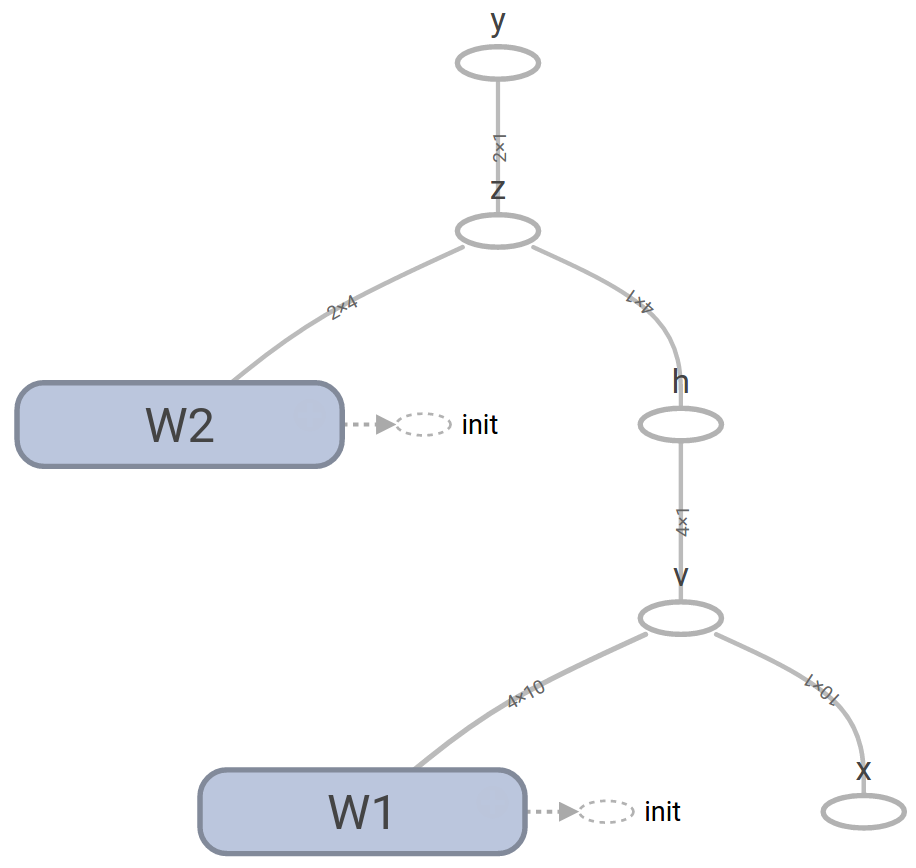
\includegraphics[scale=0.255]{images/basic_tf_graph.png}
\end{center}
\end{frame}


\begin{frame}[fragile]{Computational Graphs}
\begin{figure}[ht!]
\centering

\scalebox{1.2}{
\begin{tikzpicture}[auto]

% operations =============================

% nodes on the left
\node[op] (W1) {$\vect{W}_{1}$};
\node[textonly, below=20pt of W1] (inv1) {};
\node[op, right=30pt of inv1] (v) {$\vect{v}$};
\node[op, below right=30.5pt of v] (x) {$\vect{x}$};
\node[op, above=30.5pt of v] (hprime) {$\vect{h}^{\prime}$};
\node[textonly, above right=2pt of hprime] (h) {{\LARGE$\vect{h}$}};


%% namedscope in the left
\begin{scope}[on background layer]
\coordinate (p1) at (hprime.north);
\coordinate (p2) at (v.south east);
\coordinate (p3) at (W1.west);
\tkzCircumCenter(p1,p2,p3)
\tkzGetPoint{O}
\tkzDrawCircle[draw=orange, line width=1.5pt, fill=orange!60](O,p1)
\end{scope}

% edges on the left
\path[tedge] (W1) -- (v);
\path[tedge] (x) -- (v);
\path[tedge] (v) -- (hprime);

% nodes on the right
\node[op, right=30pt of x] (hh) {$\vect{h}$};
\node[op, above right=30.5pt of hh] (z) {$\vect{z}$};
\node[op, above=30.5pt of z] (yprime) {$\vect{y}^{\prime}$};
\node[textonly, right=30pt of z] (inv2) {};
\node[op, above=20pt of inv2] (W2) {$\vect{W}_{2}$};
\node[textonly, above left=1pt of yprime] (yhat) {{\LARGE$\hat{\vect{y}}$}};


%% namedscope in the right
\begin{scope}[on background layer]
\coordinate (p1) at (yprime.north);
\coordinate (p2) at (W2.north east);
\coordinate (p3) at (z.south west);
\tkzCircumCenter(p1,p2,p3)
\tkzGetPoint{O}
\tkzDrawCircle[draw=orange, line width=1.5pt, fill=orange!60](O,p1)
\end{scope}



% edges on the right
\path[tedge] (W2) -- (z);
\path[tedge] (hh) -- (z);
\path[tedge] (z) -- (yprime);


\end{tikzpicture}
} % scalebox
\end{figure}

\end{frame}

\begin{frame}[fragile]{Computational Graphs}
\begin{figure}[ht!]
\centering

\scalebox{1.5}{
\begin{tikzpicture}[auto]

% operations =============================
\node[op] (h) {$\vect{h}$};
\node[op, above=30pt of h] (y) {$\hat{\vect{y}}$};
\node[op, below=30pt of h] (x) {$\vect{x}$};


% edges
\path[tedge] (x) -- (h);
\path[tedge] (h) -- (y);

\end{tikzpicture}
} % scalebox
\end{figure}

\end{frame}



\begin{frame}[fragile]{Tensorflow graph}
\begin{minted}[linenos]{python}
graph = tf.Graph() 
with graph.as_default():
    with tf.variable_scope("x"):
        x_prime = tf.placeholder(shape=input_shape,
                                 dtype="float32") 

    with tf.variable_scope("h"):
        W1 = tf.get_variable(initializer=W1init)
        v = tf.matmul(W1, x_prime)
        h_prime = tf.sigmoid(v)

    with tf.variable_scope("yhat"):
        W2 = tf.get_variable(initializer=W2init)
        z = tf.matmul(W2, h_prime)
        y_prime = tf.nn.softmax(z)
\end{minted}
\end{frame}

\begin{frame}[fragile]{Tensorboard visualization}
\begin{center}
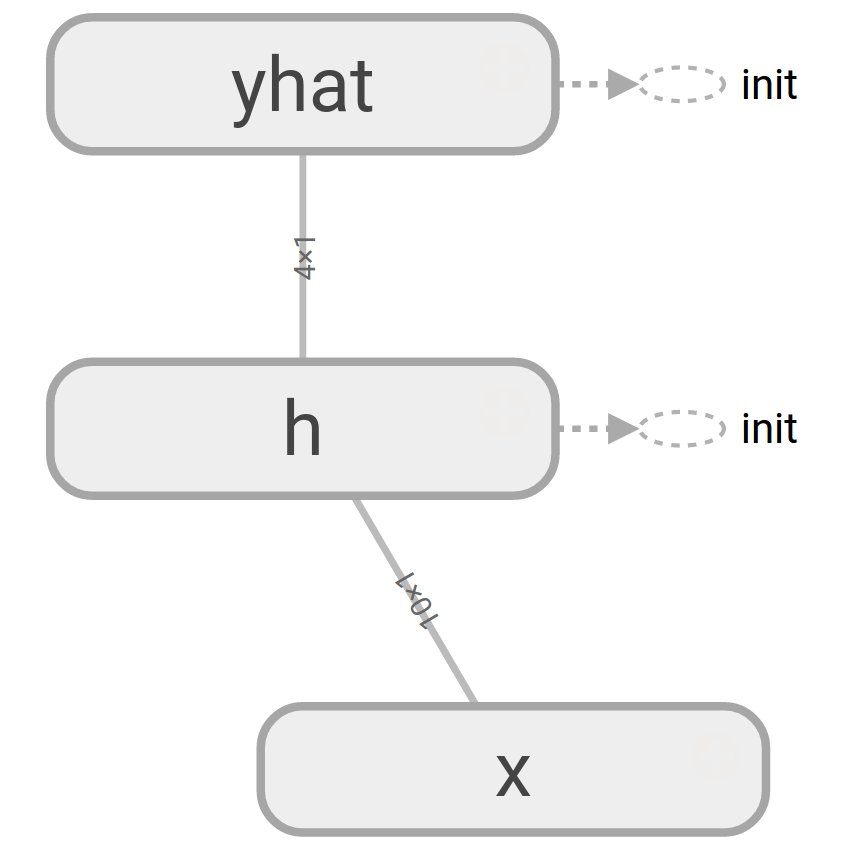
\includegraphics[scale=0.27]{images/abstract_tf_graph1.png}
\end{center}
\end{frame}

\begin{frame}[fragile]{Tensorboard visualization}
\begin{center}
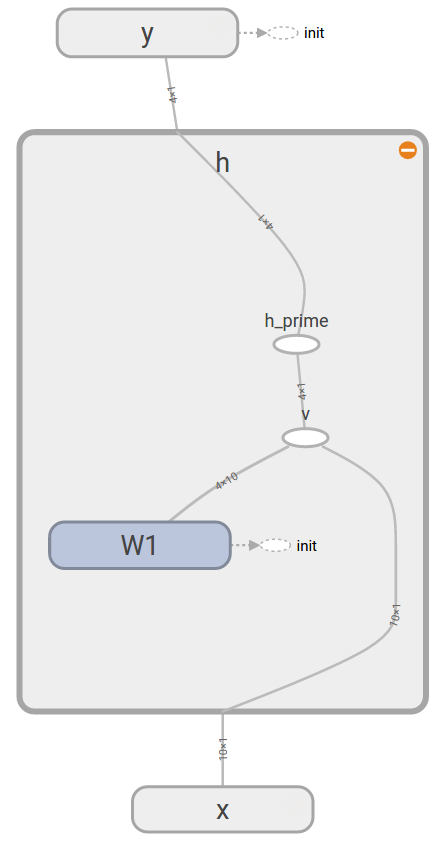
\includegraphics[scale=0.26]{images/abstract_tf_graph2.png}
\end{center}
\end{frame}


\section{RNN: the model}

\begin{frame}{RNN as a graph}
\begin{figure}[ht!]
\centering

\scalebox{0.75}{
\begin{tikzpicture}[auto]

% RNN state cell =============================
\node[state] (hprime) {$\vect{h}^{\prime}$};
\node[op, below=15pt of hprime] (a) {$\vect{a}$};

\node[op, right=25pt of a] (b) {$\vect{b}$};
\node[noop, below left=10pt and 10pt of a] (noop-left) {};
\node[state, below left=12pt and 0.1pt of noop-left] (h) {$\vect{h}$};
\node[op, above left=8pt and 15pt of noop-left] (W) {$\vect{W}$};

\node[noop, below right=10pt and 10pt of a] (noop-right) {};
\node[op, below right=12pt and 0.05pt of noop-right] (U) {$\vect{U}$};


% outer operations
\node[op, below=75pt of a] (x) {$\vect{x}$};

%% namedscope
\begin{scope}[on background layer]
\coordinate (p1) at (hprime.north);
\coordinate (p2) at (U.south east);
\coordinate (p3) at (h.south west);
\tkzCircumCenter(p1,p2,p3)
\tkzGetPoint{O}
\tkzDrawCircle[draw=orange, line width=1.5pt, fill=orange!60](O,p1)
\end{scope}

% edges

\path[tedge] (a) edge node[below right= -7pt] {$\;\; \Large{\sigma}$}  (hprime);
\path[tedge] (b) -- (a);
\path[tedge] (noop-left) -- (a);
\path[tedge] (noop-right) -- (a);
\path[tedge] (W) -- (noop-left);
\path[tedge] (h.north) to [bend left, out=70, distance=5pt] (noop-left.west);
\path[tedge] (U.north) to [bend right, out=-50, distance=5pt] (noop-right.east);
\path[tedge] (x) -- (noop-right);

% RNN output cell =============================

% operations
\node[noop, above=25pt of hprime] (noop-center) {};
\node[op, above=50pt of hprime] (o) {$\vect{o}$};
\node[op, right=15pt of o] (c) {$\vect{c}$};
\node[op, above=15pt of o] (yhat) {$\hat{\textbf{y}}$};
\node[op, below left=1pt and 10pt of o] (V) {$\vect{V}$};

% paths
\path[tedge] (hprime) -- (noop-center);
\path[tedge] (o) edge node[below right= -10pt] {$\;\;$softmax} (yhat);
\path[tedge] (c) -- (o);
\path[tedge] (V) -- (noop-center);
\path[tedge] (noop-center) -- (o);

% namedscope
\begin{scope}[on background layer]
\coordinate (p4) at (yhat.north);
\coordinate (p5) at (V.south west);
\coordinate (p6) at (c.east);
\tkzCircumCenter(p4,p5,p6)
\tkzGetPoint{O}
\tkzDrawCircle[draw=orange, line width=1.5pt, fill=orange!60](O,p4)
\end{scope}

\end{tikzpicture}
} % scalebox
\end{figure}

\end{frame}

\begin{frame}{RNN as a graph}
\begin{figure}[ht!]
\centering

\scalebox{1.40}{
\begin{tikzpicture}[auto]

% RNN state cell =============================
\node[state] (h) {$\vect{h}$};
\node[op, below=30pt of h] (x) {$\vect{x}$};
\node[op, above=30pt of h] (yhat) {$\hat{\vect{y}}$};



% edges
\path[tedge] (x) edge node[below right= -4pt] {$\vect{U}$}  (h) ;
\path[tedge] (h) edge [out=-400,in=-320,looseness=8, distance=125pt] node[above right] {$\vect{W}$} (h);
\path[tedge] (h) edge node[below right = -4pt] {$\vect{V}$} (yhat);


\end{tikzpicture}
} % scalebox
\end{figure}

\end{frame}


\begin{frame}{Definition}
A RNN is a function $f$ with two inputs:
\vspace{0.2cm}
\begin{itemize}
\item An input vector $\vect{x}$.
\vspace{0.1cm}
\item A hidden vector $\vect{h}$ representing a summary of all past inputs, called \alert{state} or \alert{cell state}.
\end{itemize}

\vspace{0.2cm}
Both inputs have a time step index $t$. The hidden unit has a recurrent definition:
\vspace{0.2cm}
\Large{
\begin{equation*}
\vect{h}^{(t)} = g(\vect{h}^{(t-1)}, \vect{x}^{(t)}; \vect{\theta})
\end{equation*}
}
\end{frame}

%"When the recurrent network is trained to perform a task that requeires predicting the future form the past, the network typically learn to use $h^{(t)}$ as a kind of lossy sumary of the task-relevant aspects of the past sequence inputs up to t"(DPB p.366)

\begin{frame}{Using our example as a concrete case}

\Large{
 \vspace{0.2cm}
\begin{equation*}
f(\vect{x}^{(t)}, \vect{h}^{(t-1)}; \vect{V}, \vect{W}, \vect{U}, \vect{c}, \vect{b}) = \vect{\hat{y}}^{(t)}
\end{equation*}
 \vspace{0.2cm}
\begin{equation*}
\vect{\hat{y}}^{(t)} = softmax(\vect{V} \vect{h}^{(t)} + \vect{c})
\end{equation*}
\vspace{0.2cm}
 \begin{equation*}
\vect{h}^{(t)} = g(\vect{h}^{(t-1)}, \vect{x}^{(t)}; \vect{W},\vect{U}, \vect{b})
\end{equation*}
\vspace{0.2cm}
\begin{equation*}
\vect{h}^{(t)} = \sigma(\vect{W} \vect{h}^{(t-1)} + \vect{U} \vect{x}^{(t)} + \vect{b})
\end{equation*}
}

\end{frame}

\begin{frame}{Unfolding the state equation}
For a finite number of steps $\tau$, the recurrent definition can be unfolded. 
For example when $\tau =3$:
\vspace{0.2cm}
\Large{
\begin{align*}
\vect{h}^{(3)}& = g(\vect{h}^{(2)}, \vect{x}^{(3)}; \vect{\theta})\\
 & = g(g(\vect{h}^{(1)}, \vect{x}^{(2)}; \vect{\theta}), \vect{x}^{(3)}; \vect{\theta})\\
 & = g(g(g(\vect{h}^{(0)}, \vect{x}^{(1)}; \vect{\theta}), \vect{x}^{(2)}; \vect{\theta}), \vect{x}^{(3)}; \vect{\theta})\\
\end{align*}
}
\end{frame}

\begin{frame}{Unfolding the graph}
% RNN STATE CELL ====================================
\newcommand{\rnnSimple}[4]{

% operations
\node[state, minimum size=40pt,#4] (h#3) {$\vect{h}^{#1}$};
\node[op, minimum size=40pt,below=30pt of h#3] (x#3) {$\vect{x}^{#1}$};
\node[op, minimum size=40pt, above=30pt of h#3] (yhat#3) {$\hat{\vect{y}}^{#1}$};

% edges
\path[tedge] (x#3) edge node[below right= -4pt] {$\vect{U}$} (h#3);
\path[tedge] (h#3) edge node[below right = -4pt] {$\vect{V}$} (yhat#3);
}

\begin{figure}[ht!]
\hspace*{-1.0cm}
\scalebox{0.9}{
\begin{tikzpicture}[auto]

% timestep 1
\rnnSimple{(1)}{(0)}{t1}{}

% % timestep 0
\node[state, minimum size=40pt,left=50pt of ht1] (ht0) {$\vect{h}^{(0)}$};

% % timestep 2
\rnnSimple{(2)}{(1)}{t2}{right=50pt of ht1};


% % timestep 2
\rnnSimple{(3)}{(1)}{t3}{right=50pt of ht2};


% % state transfers
\path[tedge] (ht0) edge node[above right = 2pt] {$\vect{W}$} (ht1);
\path[tedge] (ht1) edge node[above right = 2pt] {$\vect{W}$} (ht2);
\path[tedge] (ht2) edge node[above right = 2pt] {$\vect{W}$} (ht3);

\end{tikzpicture}
}%\scalebox
\end{figure}


\end{frame}

\section{Language model}

\begin{frame}{Definition}
We call \alert{language model} a probability distribution over sequences of tokens in a natural language.

\[
P(x_1,x_2,x_3,x_4) = p
\]

\textbf{Used for}:
\begin{itemize}
\item speech recognition
\item machine translation
\item text auto-completion
\item spell correction
\item question answering
\item summarization
\end{itemize}


\end{frame}

\begin{frame}{How do we build these probabilities?}
Using the chain rule of probability: 

\begin{equation*}
P(x_1,x_2,x_3,x_4) = P(x_1)P(x_2\vert x_1)P(x_3\vert x_1x_2)P(x_4\vert x_1x_2x_3)
\end{equation*}

\vspace{0.3cm}

To make things simple we use a \textbf{Markovian assumption}, i.e., for a specific $n$ we assume that:

\begin{equation*}
P(x_1, \dots, x_T) = \prod_{t=1}^{T} P(x_t \vert x_1, \dots, x_{t-1}) = \prod_{t=1}^{T} P(x_{t} \vert x_{t - (n+1)}, \dots, x_{t-1})
\end{equation*}	

\end{frame}

\begin{frame}{Models based on $n$-gram statistics}
The choice of $n$ yields different models.\\

\textbf{Unigram} language model ($n=1$): 
\begin{equation*}
P_{uni}(x_1, x_2, x_3, x_4) = P(x_1)P(x_2)P(x_3)P(x_4)
\end{equation*}

where $P(x_i) = count(x_i)$.\\

\textbf{Bigram} language model ($n=2$): 
\begin{equation*}
P_{bi}(x_1,x_2,x_3,x_4) = P(x_1)P(x_2\vert x_1)P(x_3\vert x_2)P(x_4\vert x_3)
\end{equation*}	
where
\[
P(x_i\vert x_j) = \frac{count(x_i, x_j)}{count(x_j)}
\]
\end{frame}

\begin{frame}{$n$-gram statistics}
\url{https://books.google.com/ngrams}
\vspace{0.4cm}

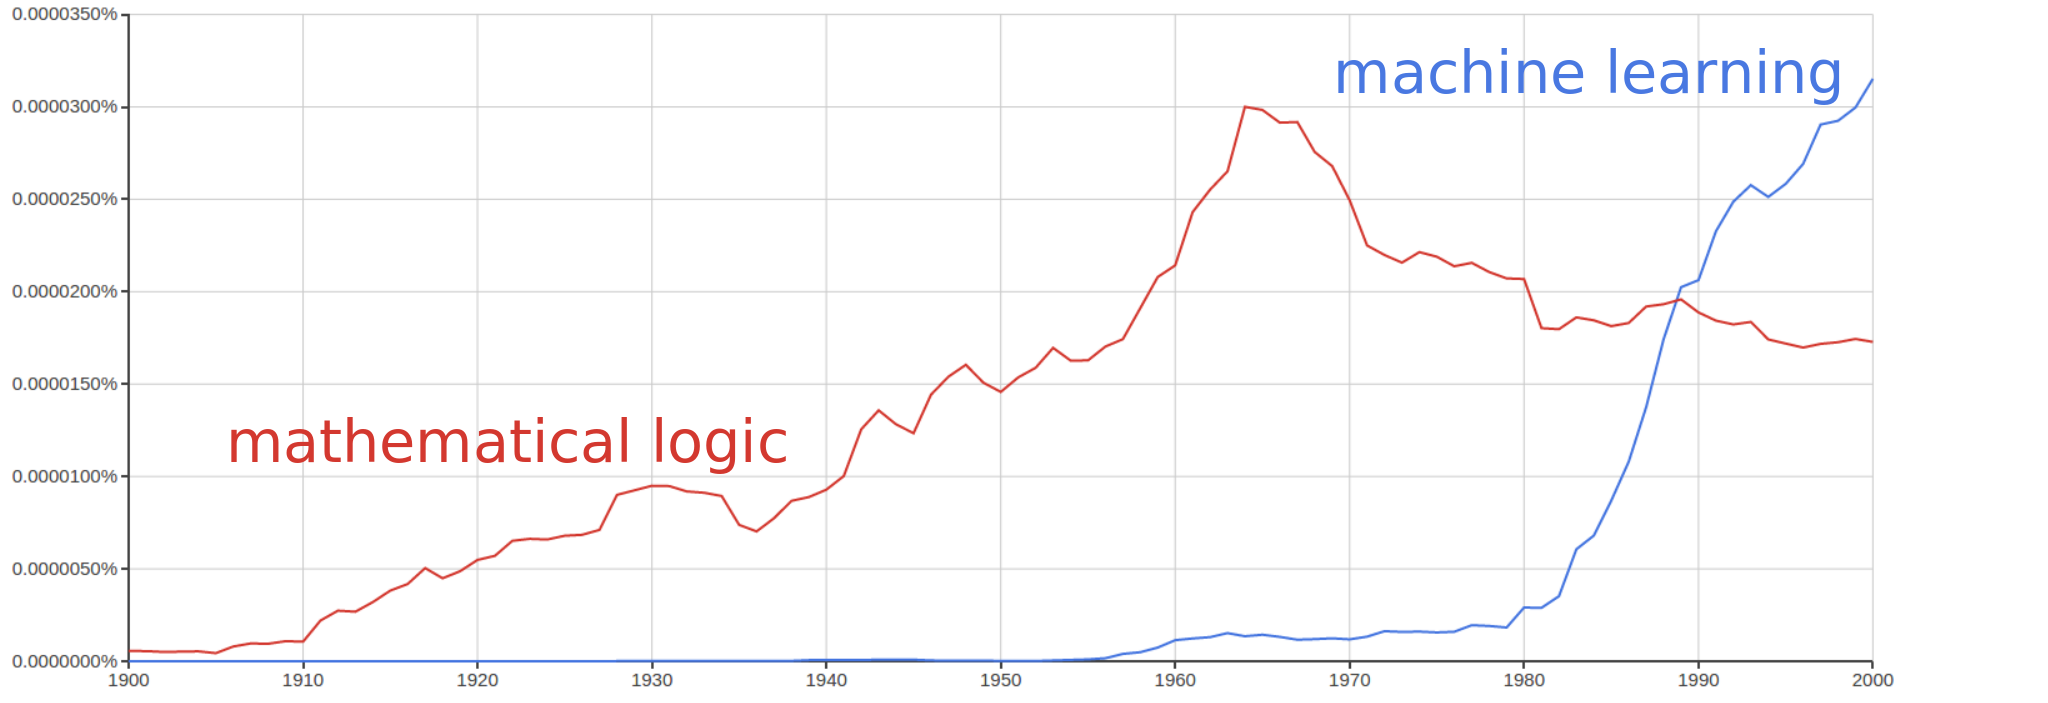
\includegraphics[scale=0.17]{images/mlXml.png}
\end{frame}



\begin{frame}{Evaluating a language model}

\begin{itemize}
\item \textbf{extrinsic task}: How our model perform in a NLP task such as text auto-completion.
\begin{itemize}
\item Time consuming.
\end{itemize}
\vspace{0.5cm}
\item \textbf{intrinsic evaluation}: perplexity.
\begin{itemize}
\item It works only when the test data is very similar to the training data.
\end{itemize}
\end{itemize}
\end{frame}

\begin{frame}{Perplexity}
\alert{Perplexity (PP)} can be thought as the weighted average branching factor of a language.\\


Given $C= x_1, x_2, \dots, x_T$, we define the perplexity of $C$ as:

\begin{align*}
PP(C) &= P(x_1, x_2, \dots, x_T)^{-\frac{1}{T}}\\
	  & \\
      &= \sqrt[T]{\frac{1}{P(x_1, x_2, \dots, x_T)}}\\
      & \\
      &= \sqrt[T]{\prod_{i=1}^{T}\frac{1}{P(x_i \vert x_1,\dots, x_{i-1})}}
\end{align*}
\end{frame}

\begin{frame}{Models based on $n$-gram statistics}
\begin{itemize}
\item Higher $n$-grams yields better performance.
\vspace{0.7cm}
\item Higher $n$-grams requires a lot of memory!
\vspace{0.1cm}
\begin{quote}
"Using one machine \alert{with 140 GB
RAM for 2.8 days}, we built an unpruned
model on 126 billion tokens."
\end{quote}
\begin{itemize}
\item [] \textit{Scalable Modified Kneser-Ney Language Model Estimation} by Heafield et al.
\end{itemize}
\end{itemize}
\end{frame}



\begin{frame}{Languagem model as sequential data prediction}
Instead of using one approach that is specific for the language domain, we can use a general model for sequential data prediction: a \textbf{RNN}. \\

Our learning task is to estimate the probability distribution 

\[
P(x_{n} = \text{word}_{j^{*}} | x_{1}, \dots ,x_{n-1})
\]

for any $(n-1)$-sequence of words $x_{1}, \dots ,x_{n-1}$.
\end{frame}

\begin{frame}{Building the dataset}
We start with a corpus $C$ with $T$ tokens and a vocabulary $\Vocab$.\\\

Example: \textbf{Meditations in an Emergency} by Frank O'Hara.\\

\begin{quote}
\alert{Am I to become profligate as if I were a blonde? Or religious as if I were French?\\
Each time my heart is broken it makes me feel more adventurous ... \\}
\end{quote}

\begin{itemize}
\item $T = 645$
\item $|\Vocab| = 347$
\end{itemize}

\end{frame}

\begin{frame}{Building the dataset}
The dataset is a collection of pairs $(\vect{x},\vect{y})$ where $\vect{x}$ is one word and $\vect{y}$ is the immediately next word. For example:
\begin{itemize}
\item [] $(\vect{x}^{(1)}, \vect{y}^{(1)}) =$ (Am, I).
\item [] $(\vect{x}^{(2)}, \vect{y}^{(2)}) =$ (I, to)
\item [] $(\vect{x}^{(3)}, \vect{y}^{(3)}) =$ (to, become)
\item [] $(\vect{x}^{(3)}, \vect{y}^{(3)}) =$ (become, profligate)
\item [] $(\vect{x}^{(4)}, \vect{y}^{(4)}) =$ (profligate, as)
\item [] $(\vect{x}^{(5)}, \vect{y}^{(5)}) =$ (as, if)
\item [] $(\vect{x}^{(6)}, \vect{y}^{(6)}) =$ (if, I)
\item [] $\dots$
\end{itemize}
\end{frame}

\begin{frame}{Notation}
\begin{itemize}
\item $\vect{E} \in \mathbb{R}^{d,|\Vocab|}$ is the matrix of word embeddings.
\vspace{0.3cm}
\item $\vect{x}^{(t)} \in \mathbb{R}^{|\Vocab|}$ is one-hot word vector at time step $t$.
\vspace{0.3cm}
\item $\vect{y}^{(t)} \in \mathbb{R}^{|\Vocab|}$ is the ground truth at time step $t$ (also an one-hot word vector).
\end{itemize}
\end{frame}

\begin{frame}{Recap: selecting word embeddings}
\Large{
\begin{align*}
  \vect{e} &= \vect{E}   \begin{bmatrix}
                         0\\
                         0\\
                         \vdots \\
                         1\\
                         \vdots \\
                         0
                         \end{bmatrix}\\         
			&= \vect{E}_{:,\;j}
\end{align*}
 }
\end{frame}


\begin{frame}{The language model: graph}
\begin{figure}[ht!]
\centering

\scalebox{0.55}{
\begin{tikzpicture}[auto]


% RNN state cell =============================
\node[state] (hprime) {$\vect{h}^{\prime}$};
\node[op, below=15pt of hprime] (a) {$\vect{a}$};

\node[op, right=25pt of a] (b) {$\vect{b}$};
\node[noop, below left=10pt and 10pt of a] (noop-left) {};
\node[state, below left=12pt and 0.1pt of noop-left] (h) {$\vect{h}$};
\node[op, above left=8pt and 15pt of noop-left] (W) {$\vect{W}$};

\node[noop, below right=10pt and 10pt of a] (noop-right) {};
\node[op, below right=12pt and 0.05pt of noop-right] (U) {$\vect{U}$};


% Input layer =============================
\node[op, below=75pt of a] (e) {$\vect{e}$};
\node[op, below left=10pt and 10pt of e] (x) {$\vect{x}$};
\node[op, below right=10pt and 10pt of e] (E) {$\vect{E}$};

%% namedscope
\begin{scope}[on background layer]
\coordinate (p1) at (hprime.north);
\coordinate (p2) at (U.south east);
\coordinate (p3) at (h.south west);
\tkzCircumCenter(p1,p2,p3)
\tkzGetPoint{O}
\tkzDrawCircle[draw=orange, line width=1.5pt, fill=orange!60](O,p1)
\end{scope}

% edges

\path[tedge] (a) edge node[below right= -7pt] {$\;\; \Large{\sigma}$}  (hprime);
\path[tedge] (b) -- (a);
\path[tedge] (noop-left) -- (a);
\path[tedge] (noop-right) -- (a);
\path[tedge] (W) -- (noop-left);
\path[tedge] (h.north) to [bend left, out=70, distance=5pt] (noop-left.west);
\path[tedge] (U.north) to [bend right, out=-50, distance=5pt] (noop-right.east);
\path[tedge] (x) -- (e);
\path[tedge] (E) -- (e);
\path[tedge] (e) -- (noop-right);

% RNN output cell =============================

% operations
\node[noop, above=25pt of hprime] (noop-center) {};
\node[op, above=50pt of hprime] (o) {$\vect{o}$};
\node[op, right=15pt of o] (c) {$\vect{c}$};
\node[op, above=15pt of o] (yhat) {$\hat{\textbf{y}}$};
\node[op, below left=1pt and 10pt of o] (V) {$\vect{V}$};

% paths
\path[tedge] (hprime) -- (noop-center);
\path[tedge] (o) edge node[below right= -10pt] {$\;\;$softmax} (yhat);
\path[tedge] (c) -- (o);
\path[tedge] (V) -- (noop-center);
\path[tedge] (noop-center) -- (o);

% namedscope
\begin{scope}[on background layer]
\coordinate (p4) at (yhat.north);
\coordinate (p5) at (V.south west);
\coordinate (p6) at (c.east);
\tkzCircumCenter(p4,p5,p6)
\tkzGetPoint{O}
\tkzDrawCircle[draw=orange, line width=1.5pt, fill=orange!60](O,p4)
\end{scope}

%% namedscope
\begin{scope}[on background layer]
\coordinate (p7) at (e.north);
\coordinate (p8) at (E.east);
\coordinate (p9) at (x.west);
\tkzCircumCenter(p7,p8,p9)
\tkzGetPoint{O}
\tkzDrawCircle[draw=orange, line width=1.5pt, fill=orange!60](O,p7)
\end{scope}


\end{tikzpicture}
} % scalebox
\end{figure}

\end{frame}

\begin{frame}{The language model: graph}
\begin{figure}[ht!]
\centering

\scalebox{1.40}{
\begin{tikzpicture}[auto]

% RNN state cell =============================
\node[state] (h) {$\vect{h}$};
\node[op, below=30pt of h] (e) {$\vect{e}$};
\node[op, above=30pt of h] (yhat) {$\hat{\vect{y}}$};



% edges
\path[tedge] (e) edge node[below right= -4pt] {$\vect{U}$}  (h) ;
\path[tedge] (h) edge [out=-400,in=-320,looseness=8, distance=125pt] node[above right] {$\vect{W}$} (h);
\path[tedge] (h) edge node[below right = -4pt] {$\vect{V}$} (yhat);


\end{tikzpicture}
} % scalebox
\end{figure}

\end{frame}



\begin{frame}{The language model: equations}
\Large{
 \vspace{0.2cm}
\begin{equation*}
\vect{e}^{(t)} = \vect{E}\vect{x}^{(t)}
\end{equation*}
\vspace{0.2cm}
 \begin{equation*}
\vect{h}^{(t)} = \sigma(\vect{W}\vect{h}^{(t-1)}+ \vect{U}\vect{e}^{(t)}+ \vect{b})
\end{equation*}
\vspace{0.2cm}
\begin{equation*}
\vect{\hat{y}}^{(t)} = softmax(\vect{V}\vect{h}^{(t)} + \vect{c})
\end{equation*}
}
\end{frame}


\begin{frame}{The Language model: unfolding example}
% RNN STATE CELL ====================================
\newcommand{\rnnSimple}[4]{

% operations
\node[state, minimum size=40pt,#4] (h#3) {$\vect{h}^{#1}$};
\node[op, minimum size=40pt, above=30pt of h#3] (yhat#3){$\hat{\vect{y}}^{#1}$};
\node[op, minimum size=40pt,below=30pt of h#3] (e#3) {$\vect{e}^{#1}$};
\node[textonly, below=0.1pt of e#3] {{\Large#2}};

% edges
\path[tedge] (e#3) edge node[below right= -4pt] {$\vect{U}$} (h#3);
\path[tedge] (h#3) edge node[below right = -4pt] {$\vect{V}$} (yhat#3);
}

\begin{figure}[ht!]
\hspace*{-1.0cm}
\scalebox{0.6}{
\begin{tikzpicture}[auto]

% timestep 1
\rnnSimple{(1)}{Am}{t1}{}

% % timestep 0
\node[state, minimum size=40pt,left=50pt of ht1] (ht0) {$\vect{h}^{(0)}$};

% % timestep 2
\rnnSimple{(2)}{I}{t2}{right=50pt of ht1};


% % timestep 2
\rnnSimple{(3)}{to}{t3}{right=50pt of ht2};


% % state transfers
\path[tedge] (ht0) edge node[above right = 2pt] {$\vect{W}$} (ht1);
\path[tedge] (ht1) edge node[above right = 2pt] {$\vect{W}$} (ht2);
\path[tedge] (ht2) edge node[above right = 2pt] {$\vect{W}$} (ht3);

% text
\node[textonly, above=40pt of yhatt2] (result) {{\Large $P(x^{(4)}| \text{Am, I, to})$}};

% Arrow to result
%  \path[tedge] (yhatt3)  edge node[bend right, out=-50, distance=25pt] (result);
\draw[->, line width=1mm] [bend right, out=-50, distance=25pt](yhatt3.north) to  (result.east);
%  \path[tedge] (yhatt3.north) to [bend right, out=-50, distance=25pt] (result.east);


\end{tikzpicture}
}%\scalebox
\end{figure}


\end{frame}

\begin{frame}{Recap: cross entropy}
\Large{
\begin{equation*}
CE(\vect{y},\vect{\hat{y}}) = -\sum_{i}\vect{y}_{i}\log(\vect{\hat{y}}_{i})  
\end{equation*}
}
\end{frame}

\begin{frame}{Loss function}
At each time $t$ the point-wise loss is:

\vspace{0.2cm}

\begin{align*}
L^{(t)} &= CE(\vect{y}^{(t)},\vect{\hat{y}}^{(t)})\\
		&= - \log(\vect{\hat{y}}_{j^{*}})\\
        &= - \log P(x^{(t+1)} = \text{word}_{j^{*}}|x^{(1)}, \dots, x^{(t)})
\end{align*}

 \vspace{0.2cm}

For example:
\begin{equation*}
L^{(3)}=- \log P(x^{(4)} = \text{become}| \text{Am}, \text{I}, \text{to})
\end{equation*}
\end{frame}


\begin{frame}{Loss function}
The loss $L$ is the mean of all the point-wise losses
\begin{equation*}
L=\frac{1}{T}\sum_{t=1}^{T}L^{(t)}
\end{equation*}

To give a concrete example, let's take the first sentence of the poem as $C$:
\begin{quote}
\alert{Am I to become profligate as if I were a blonde?}
\end{quote}

\begin{itemize}
\item $T = 12$
\item $|\Vocab| = 11$
\end{itemize}

\end{frame}


\begin{frame}{Loss function: example}

\begin{align*}
        L &=-\frac{1}{12}[\log P(\text{Am} | <\text{eos}>)\\
          &+ \log P(\text{I} | \text{Am})\\
          &+ \log P(\text{to}| \text{Am}, \text{I})\\
          &+ \log P(\text{become}| \text{Am}, \text{I}, \text{to})\\
		  &+ \log P(\text{profligate}| \text{Am}, \text{I}, \text{to}, \text{become})\\
          &+ \log P(\text{as}| \text{Am}, \text{I}, \text{to}, \text{become}, \text{profligate})\\
          &+ \log P(\text{if}| \text{Am}, \text{I}, \text{to}, \text{become}, \text{profligate}, \text{as})\\
          &+ \log P(\text{I}| \text{Am}, \text{I}, \text{to}, \text{become}, \text{profligate}, \text{as}, \text{if})\\
          &+ \log P(\text{were}| \text{Am}, \text{I}, \text{to}, \text{become}, \text{profligate}, \text{as}, \text{if}, \text{I})\\
          &+ \log P(\text{a}| \text{Am}, \text{I}, \text{to}, \text{become}, \text{profligate}, \text{as}, \text{if}, \text{I}, \text{were})\\
          &+ \log P(\text{blonde}| \text{Am}, \text{I}, \text{to}, \text{become}, \text{profligate}, \text{as}, \text{if}, \text{I}, \text{were}, \text{a})\\
          &+ \log P(<\text{eos}>| \text{Am}, \text{I}, \text{to}, \text{become}, \text{profligate}, \text{as}, \text{if}, \text{I}, \text{were}, \text{a}, \text{blonde})]
\end{align*}

\end{frame}

\begin{frame}{Loss and Perplexity}
Since
\begin{align*}
L^{(t)} & = - \log P(x^{(t+1)} |x^{(1)}, \dots, x^{(t)})\\
& =  \log(\frac{1}{P(x^{(t+1)}|x^{(1)}, \dots, x^{(t)})})\\
\end{align*}
We have that:

\begin{align*}
        L &=\frac{1}{T} \sum_{t=1}^{T} L^{(t)}\\
          &= \log\left( \sqrt[T]{\prod_{i=1}^{T}\frac{1}{P(x_i \vert x_1,\dots, x_{i-1})}} \right)\\
          &= \log(PP(C))
\end{align*}
\end{frame}

\begin{frame}{Loss and Perplexity}
So another definition of perplexity is
\vspace{0.5cm}
\Large{
\begin{equation*}
2^{L} = PP(C)
\end{equation*}
}
\end{frame}

\section{Back Propagation}

\begin{frame}{Chain rule of Calculus}
\Large{
\begin{itemize}
\item $x \in \mathbb{R}$
\item $f:\mathbb{R} \rightarrow\mathbb{R}$, $g:\mathbb{R} \rightarrow\mathbb{R}$. 
\item $y = g(x)$
\item $z = f(g(x)) = f(y)$
\end{itemize}

\[
\frac{dz}{dx} = \frac{dz}{dy} \frac{dy}{dx} 
\]
}
\end{frame}

\begin{frame}{Chain rule: example}
\Large{
\begin{itemize}
\item $y = x^2$

\vspace{0.3cm}

\item $z = \log(y)$
\end{itemize}

\vspace{0.5cm}

\[
\frac{dz}{dx} = \frac{dz}{dy} \frac{dy}{dx} = \frac{1}{x^2}2x = \frac{2}{x}
\]
}
\end{frame}

\begin{frame}{Chain rule = graph}
\begin{figure}[ht!]
\centering

\scalebox{1.0}{
\begin{tikzpicture}[auto]

% operations =============================
\node[op] (y) {y};
\node[op, above=30pt of y] (z) {z};
\node[op, below=30pt of y] (x) {x};

% gradients =============================
\visible<2->{\node[gradient, right=50pt of z] (delzdely) {$\frac{dz}{dy}$};}
\visible<2->{\node[textonly, right=0.1pt of delzdely] {$=\frac{1}{x^{2}}$};}
\visible<3->{\node[gradient, right=50pt of y] (delydelx) {$\frac{dy}{dx}$};}
\visible<3->{\node[textonly, right=0.1pt of delydelx] {$=2x$};}
\visible<4->{\node[gradient, right=80pt of x] (delzdelx) {$\frac{dz}{dx}$};}
\visible<4->{\node[textonly, right=0.1pt of delzdelx] {$=\frac{2}{x}$};}


% edges
\path[tedge] (x) -- (y);
\path[tedge] (y) -- (z);
\visible<2->{\path[tedge] (z) -- (delzdely);}
\visible<3->{\path[tedge] (y) -- (delydelx);}
\visible<4->{\path[tedge] (x) -- (delzdelx);}
\visible<4->{\path[tedge] (delydelx) -- (delzdelx);}
\visible<4->{\path[tedge] (delzdely) to [bend right, out=-310, in=100, distance=40pt] (delzdelx);}


% \visible<2->{\node[gradient, left=20pt of V] (grad-V) {$\nabla_{\textbf{V}}\textbf{L}$};}


\end{tikzpicture}
} % scalebox
\end{figure}

\end{frame}

\begin{frame}{Chain rule: vector notation}
\Large{
\begin{itemize}
\item $\vect{x} \in \mathbb{R}^{m}$
\item $\vect{y} \in \mathbb{R}^{n}$
\item $f:\mathbb{R}^{n} \rightarrow\mathbb{R}$, $g:\mathbb{R}^{m} \rightarrow\mathbb{R}^{n}$. 
\item $\vect{y} = g(\vect{x})$
\item $\vect{z} = f(g(\vect{x})) = f(\vect{y})$
\end{itemize}
\[
\frac{\partial z}{\partial x_{i}} =\sum_{j} \frac{\partial z}{\partial y_{j}} \frac{\partial y_{j}}{\partial x_{i}} 
\]
}
\end{frame}

\begin{frame}{Chain rule: vector notation}

\Large{
\begin{itemize}
\item $\vect{x} \in \mathbb{R}^{m}$
\item $\vect{y} \in \mathbb{R}^{n}$
\item $f:\mathbb{R}^{n} \rightarrow\mathbb{R}$, $g:\mathbb{R}^{m} \rightarrow\mathbb{R}^{n}$. 
\item $\vect{y} = g(\vect{x})$
\item $\vect{z} = f(g(\vect{x})) = f(\vect{y})$
\end{itemize}
\[
\grad{\vect{x}}{z} = \left(\frac{\partial \vect{y}}{\partial \vect{x}}\right)^{T}\grad{\vect{y}}{z}
\]
}
\end{frame}

\begin{frame}{Recap: gradient}
\Large{
\begin{align*}
  \grad{\vect{y}}{z} &= \begin{bmatrix}
                         \frac{\partial z}{\partial y_{1}} \\
                         \frac{\partial z}{\partial y_{2}} \\
                         \vdots \\
                         \frac{\partial z}{\partial y_{n}}
                         \end{bmatrix}
\end{align*}
 }
\end{frame}

\begin{frame}{Recap: Jacobian matrix}
\Large{
\[
\frac{\partial \vect{y}}{\partial \vect{x}} =
\begin{bmatrix} 

\frac{\partial y_{1}}{\partial x_{1}} & \frac{\partial y_{1}}{\partial x_{2}} & \dots & \frac{\partial y_{1}}{\partial x_{m}} \\

\vdots & \ddots &\dots & \vdots \\

\frac{\partial y_{n}}{\partial x_{1}} &\frac{\partial y_{n}}{\partial x_{2}} & \dots&\frac{\partial y_{n}}{\partial x_{m}} 

\end{bmatrix}
\]
 }
\end{frame}

\begin{frame}{Chain rule: example}
\Large{
\begin{itemize}
\item $\vect{y} = \vect{W}\vect{x}$

\vspace{0.3cm}

\item $z = \vect{b}^{T}\vect{y}$
\end{itemize}

\vspace{0.5cm}

\[
\grad{\vect{x}}{z} =  \vect{W}^{T}\vect{b}
\]
}
\end{frame}


\begin{frame}{Chain rule = graph}
\begin{figure}[ht!]
\centering

\scalebox{1.0}{
\begin{tikzpicture}[auto]

% operations =============================
\node[op] (y) {$\vect{y}$};
\node[op, above=30pt of y] (z) {$z$};
\node[op, below=30pt of y] (x) {$\vect{x}$};

% gradients =============================
\visible<2->{\node[gradient, right=50pt of z] (delzdely) {$\grad{\vect{y}}{z}$};}
\visible<2->{\node[textonly, right=0.1pt of delzdely] {$=\vect{b}$};}
\visible<3->{\node[gradient, right=50pt of y] (delydelx) {$\Jacobian{\vect{y}}{\vect{x}}$};}
\visible<3->{\node[textonly, right=0.1pt of delydelx] {$=\vect{W}$};}
\visible<4->{\node[gradient, right=80pt of x] (delzdelx) {$\grad{\vect{x}}{z}$};}
\visible<4->{\node[textonly, right=0.1pt of delzdelx] {$=\dotp{\vect{W}}{\vect{b}}$};}


% edges
\path[tedge] (x) -- (y);
\path[tedge] (y) -- (z);
\visible<2->{\path[tedge] (z) -- (delzdely);}
\visible<3->{\path[tedge] (y) -- (delydelx);}
\visible<4->{\path[tedge] (x) -- (delzdelx);}
\visible<4->{\path[tedge] (delydelx) -- (delzdelx);}
\visible<4->{\path[tedge] (delzdely) to [bend right, out=-310, in=100, distance=40pt] (delzdelx);}


% \visible<2->{\node[gradient, left=20pt of V] (grad-V) {$\nabla_{\textbf{V}}\textbf{L}$};}


\end{tikzpicture}
} % scalebox
\end{figure}

\end{frame}

\begin{frame}{Computing the gradient in a RNN}
\begin{itemize}
\item We simple apply the back-propagation algorithm to the unrolled computational graph.

\vspace{0.5cm}

\item Since each subgraph represents a time step, the application of back-propagation in this model is also called \alert{Back-Propagation Through Time}.
\end{itemize}
\end{frame}


\begin{frame}{A very simple RNN}

\Large{
\begin{equation*}
\vect{a}^{(t)} = \vect{W} \vect{h}^{(t-1)} + \vect{U} \vect{x}^{(t)}
\end{equation*}

\vspace{0.1cm}

\begin{equation*}
\vect{h}^{(t)} = \sigma(\vect{a}^{(t)})
\end{equation*}

\vspace{0.1cm}

\begin{equation*}
\vect{o}^{(t)} = \vect{V} \vect{h}^{(t)}
\end{equation*}

\vspace{0.1cm}

\begin{equation*}
\vect{\hat{y}}^{(t)} = softmax(\vect{o}^{(t)})
\end{equation*}
}

\end{frame}


\begin{frame}{RNN time unfolding}
% RNN STATE CELL ====================================
\newcommand{\rnnstatecell}[4]{

% operations
\node[state, minimum size=40pt,#4] (hprime#3) {$\textbf{h}^{#1}$};
\node[op, minimum size=40pt,below=15pt of hprime#3] (a#3) {$\textbf{a}^{#1}$};

\node[noop, below left=10pt and 10pt of a#3] (noop-left#3) {};
\node[state, minimum size=40pt, below left=12pt and 0.1pt of noop-left#3] (h#3) {$\textbf{h}^{#2}$};
\node[op, above left=8pt and 15pt of noop-left#3] (W#3) {W};

\node[noop, below right=10pt and 10pt of a#3] (noop-right#3) {};
\node[op, below right=12pt and 0.05pt of noop-right#3] (U#3) {U};

% outer operations
\node[op, minimum size=40pt, below=75pt of a#3] (x#3) {$\textbf{x}^{#1}$};

%% namedscope
\begin{scope}[on background layer]
\coordinate (p1#3) at (hprime#3.north);
\coordinate (p2#3) at (U#3.south east);
\coordinate (p3#3) at (h#3.south west);
\tkzCircumCenter(p1#3,p2#3,p3#3)
\tkzGetPoint{O}
\tkzDrawCircle[draw=orange, line width=1.5pt, fill=orange!60](O,p1#3)
\end{scope}

% edges
\path[tedge] (a#3) -- (hprime#3);
\path[tedge] (noop-left#3) -- (a#3);
\path[tedge] (noop-right#3) -- (a#3);
\path[tedge] (W#3) -- (noop-left#3);
\path[tedge] (h#3.north) to [bend left, out=70, distance=5pt] (noop-left#3.west);
\path[tedge] (U#3.north) to [bend right, out=-50, distance=5pt] (noop-right#3.east);
\path[tedge] (x#3) -- (noop-right#3);
}

% RNN OUTPUT ====================================
\newcommand{\rnnoutput}[3]{

% operations
\node[op, minimum size=40pt, #3] (o#2) {$\textbf{o}^{#1}$};
\node[op, minimum size=40pt, above=15pt of o#2] (yhat#2) {$\hat{\textbf{y}}^{#1}$};
\node[op, below left=1pt and 10pt of o#2] (V#2) {$\textbf{V}$};
\node[op, minimum size=40pt, right=50pt of yhat#2] (L#2) {$\textbf{L}^{#1}$};
\node[op, minimum size=40pt, right=20pt of L#2] (y#2) {$\textbf{y}^{#1}$};

% paths
\path[tedge] (o#2) -- (yhat#2);
\path[tedge] (yhat#2) -- (L#2);
\path[tedge] (y#2) -- (L#2);
\path[tedge] (V#2.north) to [bend left, out=90, in=135, distance=10pt] (o#2.west);

% namedscope
\begin{scope}[on background layer]
\coordinate (p1#2) at (yhat#2.north);
\coordinate (p2#2) at (V#2.south west);
\coordinate [right=35pt of o#2] (p3#2);
\tkzCircumCenter(p1#2,p2#2,p3#2)
\tkzGetPoint{O}
\tkzDrawCircle[draw=orange,line width=1.5pt, fill=orange!60](O,p1#2)
\end{scope}
}

\begin{figure}[ht!]
\hspace*{-1.0cm}
\scalebox{0.45}{
\begin{tikzpicture}[auto]

% timestep 1 cell
\rnnstatecell{(1)}{(0)}{t1}{}

% timestep 2 cell
\rnnstatecell{(2)}{(1)}{t2}{right=140pt of hprimet1};

% previous cell
\rnnstatecell{(\tau-1)}{(\tau-2)}{prev}{right=200pt of hprimet2};

% next cell
\rnnstatecell{(\tau)}{(\tau-1)}{next}{right=140pt of hprimeprev}

% state transfers
\path[tedge] (hprimet1.east) to [out=10, in=-160] (ht2.west);

\coordinate[right=30pt of hprimet2] (hppp);
\path[tedge] (hppp.east) to [out=10, in=-160] (hprev.west);

\path[tedge] (hprimeprev.east) to [out=10, in=-160] (hnext.west);

% ...
\node[fill=white, right=70pt of at2] (ppp) {\Huge{$\cdots$}};

% output
\rnnoutput{(\tau)}{output}{above=50pt of hprimenext};

\path[tedge] (hprimenext) -- (ooutput);

\end{tikzpicture}
}%\scalebox
\end{figure}


\end{frame}

\begin{frame}{Recap: Hadamard product}
\Large{
\begin{equation*}
(\vect{x} \circ \vect{y})_{i} = \vect{x}_{i} \vect{y}_{i} 
\end{equation*}

\vspace{0.5cm}

\begin{equation*}
(\vect{x} \circ \vect{y}) = diag(\vect{y})\vect{x} 
\end{equation*}
 }
\end{frame}

\begin{frame}{Chain rule: RNN graph}
\begin{figure}[ht!]
\centering

\scalebox{0.71}{
\begin{tikzpicture}[auto]


% RNN state cell =============================
\node[state] (hprime) {$\myprime{\vect{h}}$};
\node[op, below=15pt of hprime] (a) {$\vect{a}$};

\node[noop, below left=10pt and 10pt of a] (noop-left) {};
\node[state, below left=12pt and 0.1pt of noop-left] (h) {$\vect{h}$};
\node[op, above left=8pt and 15pt of noop-left] (W) {$\vect{W}$};

\node[noop, below right=10pt and 10pt of a] (noop-right) {};
\node[op, below right=12pt and 0.05pt of noop-right] (U) {$\vect{U}$};

% gradients
% $\grad{\myprime{\vect{h}}}{L}$
% $\outerp{\grad{\vect{a}}{L}}{\vect{x}}=$

\visible<6->{\node[gradient, right=50pt of hprime] (grad-hprime) {$\grad{\myprime{\vect{h}}}{L}$};}
\visible<7->{\node[textonly, right=0.1pt of grad-hprime] {$=\dotpPright{\vect{V}}{\grad{\vect{o}}{L}}$};}

\visible<8->{\node[gradient, right=65pt of a] (grad-a) {$\grad{\vect{a}}{L}$};}
\visible<9->{\node[textonly, right=0.1pt of grad-a] {$=\left(\grad{\myprime{\vect{h}}}{L}\right)\circ\myprime{\vect{h}}\circ(1-\myprime{\vect{h}})$};}

\visible<10->{\node[gradient, right=40pt of U] (grad-U) {$\grad{\vect{U}}{L}$};}
\visible<11->{\node[textonly, right=0.1pt of grad-U] {$=\outerp{\grad{\vect{a}}{L}}{\vect{x}}$};}

\visible<12->{\node[gradient, left=30pt of W] (grad-W) {$\grad{\vect{W}}{L}$};}
\visible<13->{\node[textonly, left=0.1pt of grad-W] {$\outerp{\grad{\vect{a}}{L}}{\vect{h}}=$};}

\visible<14->{\node[gradient, left=30pt of h] (grad-h) {$\grad{\vect{h}}{L}$};}
\visible<15->{\node[textonly, left=0.1pt of grad-h] {$\dotpPright{\vect{W}}{\grad{\vect{a}}{L}}=$};}

% outer operations
\node[op, below=75pt of a] (x) {$\vect{x}$};

%% namedscope
\begin{scope}[on background layer]
\coordinate (p1) at (hprime.north);
\coordinate (p2) at (U.south east);
\coordinate (p3) at (h.south west);
\tkzCircumCenter(p1,p2,p3)
\tkzGetPoint{O}
\tkzDrawCircle[draw=orange, line width=1.5pt, fill=orange!60](O,p1)
\end{scope}

% edges
\visible<6->{\path[tedge] (hprime) -- (grad-hprime);}
\visible<8->{\path[tedge] (a) -- (grad-a);}
\visible<10->{\path[tedge] (U) -- (grad-U);}
\visible<12->{\path[tedge] (W) -- (grad-W);}
\visible<14->{\path[tedge] (h) -- (grad-h);}

\path[tedge] (a) -- (hprime);
\path[tedge] (noop-left) -- (a);
\path[tedge] (noop-right) -- (a);
\path[tedge] (W) -- (noop-left);
\path[tedge] (h.north) to [bend left, out=70, distance=5pt] (noop-left.west);
\path[tedge] (U.north) to [bend right, out=-50, distance=5pt] (noop-right.east);
\path[tedge] (x) -- (noop-right);

% RNN output cell =============================

% operations
\node[op, above=50pt of hprime] (o) {$\vect{o}$};
\node[op, above=15pt of o] (yhat) {$\hat{\vect{y}}$};
\node[op, below left=1pt and 10pt of o] (V) {$\vect{V}$};
\node[op, right=50pt of yhat] (L) {$L$};
\node[op, right=20pt of L] (y) {$\vect{y}$};

% gradients
\visible<4->{\node[gradient, left=20pt of V] (grad-V) {$\grad{\vect{V}}{L}$};}
\visible<2->{\node[gradient, right=50pt of o] (grad-o) {$\grad{\vect{o}}{L}$};}
\visible<3->{\node[textonly, right=0.1pt of grad-o] {$=\hat{\vect{y}}-\vect{y}$};}
\visible<5->{\node[textonly, left=0.1pt of grad-V] {$\outerp{\grad{\vect{o}}{L}}{\myprime{\vect{h}}}=$};}

% paths
\path[tedge] (hprime) -- (o);
\path[tedge] (o) -- (yhat);
\path[tedge] (yhat) -- (L);
\path[tedge] (y) -- (L);
\visible<2->{\path[tedge] (o) -- (grad-o);}
\path[tedge] (V.north) to [bend left, out=90, in=135, distance=10pt] (o.west);
\visible<4->{\path[tedge] (V) -- (grad-V);}

% namedscope
\begin{scope}[on background layer]
\coordinate (p4) at (yhat.north);
\coordinate (p5) at (V.south west);
\coordinate [right=35pt of o] (p6);
\tkzCircumCenter(p4,p5,p6)
\tkzGetPoint{O}
\tkzDrawCircle[draw=orange, line width=1.5pt, fill=orange!60](O,p4)
\end{scope}

\end{tikzpicture}
} % scalebox
\end{figure}

\end{frame}


\begin{frame}{Back Propagation Throught Time}
\newcommand{\rnnstatecell}[4]{

% operations
\node[state, minimum size=40pt,#4] (hprime#3) {$\vect{h}^{#1}$};
\node[op, minimum size=40pt,below=15pt of hprime#3] (a#3) {$\vect{a}^{#1}$};

\node[noop, below left=10pt and 10pt of a#3] (noop-left#3) {};
\node[state, minimum size=40pt, below left=12pt and 0.1pt of noop-left#3] (h#3) {$\vect{h}^{#2}$};
\node[op, above left=8pt and 15pt of noop-left#3] (W#3) {$\vect{W}$};

\node[noop, below right=10pt and 10pt of a#3] (noop-right#3) {};
\node[op, below right=12pt and 0.05pt of noop-right#3] (U#3) {$\vect{U}$};

% outer operations
\node[op, minimum size=40pt, below=75pt of a#3] (x#3) {$\vect{x}^{#1}$};

%% namedscope
\begin{scope}[on background layer]
\coordinate (p1) at (hprime#3.north);
\coordinate (p2) at (U#3.south east);
\coordinate (p3) at (h#3.south west);
\tkzCircumCenter(p1,p2,p3)
\tkzGetPoint{O}
\tkzDrawCircle[draw=orange,line width=2pt, fill=orange!60](O,p1)
\end{scope}

% edges
\path[tedge] (a#3) -- (hprime#3);
\path[tedge] (noop-left#3) -- (a#3);
\path[tedge] (noop-right#3) -- (a#3);
\path[tedge] (W#3) -- (noop-left#3);
\path[tedge] (h#3.north) to [bend left, out=70, distance=5pt] (noop-left#3.west);
\path[tedge] (U#3.north) to [bend right, out=-50, distance=5pt] (noop-right#3.east);
\path[tedge] (x#3) -- (noop-right#3);
}

\begin{figure}
\centering

\scalebox{0.42}{
\begin{tikzpicture}[auto]

% previous cell
\rnnstatecell{(\tau-1)}{(\tau-2)}{prev}{}

% past cells
\node[textonly, left=60pt of Wprev] (dots) {{\Huge $\cdots$}};

% past edge
\path[tedge] (dots) to [out=10, in=-160] (hprev.west);


% next cell
\rnnstatecell{(\tau)}{(\tau-1)}{next}{right=230pt of hprimeprev}

% state transfer
\path[tedge] (hprimeprev.east) to [out=10, in=-160] (hnext.west);

% loss
\node[op, minimum size=40pt, above right=80pt and 40pt of hprimenext] (L) {$L^{(\tau)}$};
\node[textonly, above=80pt of hprimenext] (ppp) {{\Huge $\cdots$}};

% loss edges
\path[tedge] (hprimenext.north) to [bend left, out=-110, in=100, distance=20pt] (ppp.west);
\path[tedge] (ppp) -- (L);

% gradients from time step tau 
\visible<2->{\node[gradient, above right=1pt and 70pt of hprimenext] (grad-hprime) {$\grad{\vect{h}^{(\tau)}}{L^{(\tau)}}$};}
\visible<3->{\node[textonly, right=0.1pt of grad-hprime] {$=\dotpPright{\vect{V}}{\hat{\vect{y}}^{(\tau)} - \vect{y}^{(\tau)}}$};}


\visible<4->{\node[gradient, right=65pt of anext] (grad-a) {$\grad{\vect{a}^{(\tau)}}{L^{(\tau)}}$};}
\visible<5->{\node[textonly, right=0.1pt of grad-a] {$=\left(\grad{\vect{h}^{(\tau)}}{L^{(\tau)}}\right)\circ\vect{h}^{(\tau)}\circ(1-\vect{h}^{(\tau)})$};}


\visible<6->{\node[gradient, below right=0.1pt and 40pt of Unext] (grad-U) {$\grad{\vect{U}^{(\tau)}}{L^{(\tau)}}$};}
\visible<7->{\node[textonly, right=0.1pt of grad-U] {$=\outerp{\grad{\vect{a}^{(\tau)}}{L^{(\tau)}}}{\vect{x}^{(\tau)}}$};}


\visible<8->{\node[gradient, above left=70pt and 10pt of Wnext] (grad-W) {$\grad{\vect{W}^{(\tau)}}{L^{(\tau)}}$};}
\visible<9->{\node[textonly, left=0.1pt of grad-W] {$\outerp{\grad{\vect{a^{(\tau)}}}{L^{(\tau)}}}{\vect{h}^{(\tau-1)}}=$};}


% gradients from time step tau -1
\visible<10->{\node[gradient, above left=60pt and 10pt of hprimeprev] (grad-hprimeprev) {$\grad{\vect{h}^{(\tau-1)}}{L^{(\tau)}}$};}
\visible<11->{\node[textonly, left=0.1pt of grad-hprimeprev] {$\dotpPright{\vect{W}}{\grad{\vect{a}^{(\tau)}}{L^{(\tau)}}}=$};}


\visible<12->{\node[gradient, below left=55pt and -20pt of hnext] (grad-a-prev) {$\grad{\vect{a}^{(\tau-1)}}{L^{(\tau)}}$};}
\visible<13->{\node[textonly, right=0.1pt of grad-a-prev] {$=\left(\grad{\vect{h}^{(\tau-1)}}{L^{(\tau)}}\right)\circ\vect{h}^{(\tau-1)}\circ(1-\vect{h}^{(\tau-1)})$};}


\visible<14->{\node[gradient, below left=20pt and 10pt of grad-a-prev] (grad-U-prev) {$\grad{\vect{U}^{(\tau-1)}}{L^{(\tau)}}$};}
\visible<15->{\node[textonly, left=0.1pt of grad-U-prev] {$\outerp{\grad{\vect{a}^{(\tau-1)}}{L^{(\tau)}}}{\vect{x}^{(\tau-1)}}=$};}


\visible<16->{\node[gradient, above left=70pt and 10pt of Wprev] (grad-W-prev) {$\grad{\vect{W}^{(\tau-1)}}{L^{(\tau)}}$};}
\visible<17->{\node[textonly, left=0.1pt of grad-W-prev] {$\outerp{\grad{\vect{a^{(\tau-1)}}}{L^{(\tau)}}}{\vect{h}^{(\tau-2)}}=$};}

\visible<18->{\node[gradient, below left=20pt and 10pt of hprev] (grad-hprev) {$\grad{\vect{h}^{(\tau-2)}}{L^{(\tau)}}$};}
\visible<19->{\node[textonly, left=0.1pt of grad-hprev] {$\dotpPright{\vect{W}}{\grad{\vect{a}^{(\tau-1)}}{L^{(\tau)}}}=$};}



% gradient's edges
\visible<2->{\path[tedge] (hprimenext) -- (grad-hprime);}
\visible<4->{\path[tedge] (anext) -- (grad-a);}
\visible<6->{\path[tedge] (Unext) -- (grad-U);}
\visible<8->{\path[tedge] (Wnext) -- (grad-W);}
\visible<10->{\path[tedge] (hprimeprev) -- (grad-hprimeprev);}
\visible<12->{\path[tedge] (aprev.east) to [out=10, in=-160] (grad-a-prev);}
\visible<14->{\path[tedge] (Uprev) -- (grad-U-prev);}
\visible<16->{\path[tedge] (Wprev) -- (grad-W-prev);}
\visible<18->{\path[tedge] (hprev) -- (grad-hprev);}


\end{tikzpicture}
}%\scalebox
\end{figure}


\end{frame}

\begin{frame}{Back Propagation Through Time}
The gradients on $\vect{V}$, $\vect{W}$ and $\vect{U}$ are:
\vspace{0.3cm}
\Large{
\begin{equation*}
\grad{\vect{V}}{L^{(\tau)}} = \outerp{\grad{\vect{o}^{(\tau)}}{L^{(\tau)}}}{\vect{h}^{(\tau)}} 
\end{equation*}


\begin{equation*}
\grad{\vect{W}}{L^{(\tau)}} = \sum_{t=1}^{\tau}\grad{\vect{W}^{(t)}}{L^{(\tau)}}
\end{equation*}

\begin{equation*}
\grad{\vect{U}}{L^{(\tau)}} = \sum_{t=1}^{\tau}\grad{\vect{U}^{(t)}}{L^{(\tau)}}
\end{equation*}
}
\end{frame}

\section{Vanishing or Exploding Gradient}
\begin{frame}{The problem of training RNN}
Let's calculate $\grad{\vect{U}}{L^{(3)}}$:
\begin{align*}
\grad{\vect{U}}{L^{(3)}} &= \sum_{t=1}^{3}\grad{\vect{U}^{(t)}}{L^{(3)}}\\
&= \grad{\vect{U}^{(1)}}{L^{(3)}} + \grad{\vect{U}^{(2)}}{L^{(3)}} + \grad{\vect{U}^{(3)}}{L^{(3)}}
\end{align*}
\end{frame}

\begin{frame}{Calculating $\grad{\vect{U}^{(3)}}{L^{(3)}}$ }
\begin{align*}
\grad{\vect{U}^{(3)}}{L^{(3)}} &=\outerp{\grad{\vect{a}^{(3)}}{L^{(3)}}}{\vect{x}^{(3)}}\\
%
\visible<2->{&=\outerp{\left(\grad{\vect{h}^{(3)}}{L^{(3)}}\right)\circ\vect{h}^{(3)}\circ(1-\vect{h}^{(3)})}{\vect{x}^{(3)}}\\}
%
\visible<3->{&=\outerp{\left(\dotpPright{\vect{V}}{\hat{\vect{y}}^{(3)} - \vect{y}^{(3)}}\right)\circ\vect{h}^{(3)}\circ(1-\vect{h}^{(3)})}{\vect{x}^{(3)}}\\}
\end{align*}
\end{frame}


\begin{frame}{Calculating $\grad{\vect{U}^{(2)}}{L^{(3)}}$ }
\footnotesize{
\begin{align*}
\grad{\vect{U}^{(2)}}{L^{(3)}} &=\outerp{\grad{\vect{a}^{(2)}}{L^{(3)}}}{\vect{x}^{(2)}}\\
%
\visible<2->{&=\outerp{\left(\grad{\vect{h}^{(2)}}{L^{(3)}}\right)\circ\vect{h}^{(2)}\circ(1-\vect{h}^{(2)})}{\vect{x}^{(2)}}\\}
%
\visible<3->{&=\outerp{\left(\dotpPright{\vect{W}}{\grad{\vect{a}^{(3)}}{L^{(3)}}}\right)\circ\vect{h}^{(2)}\circ(1-\vect{h}^{(2)})}{\vect{x}^{(2)}}\\}
%
\visible<4->{&=\outerp{\left(\dotpPright{\vect{W}}{\left(\grad{\vect{h}^{(3)}}{L^{(3)}}\right)\circ\vect{h}^{(3)}\circ(1-\vect{h}^{(3)})}\right)\circ\vect{h}^{(2)}\circ(1-\vect{h}^{(2)})}{\vect{x}^{(2)}}\\}
%
\visible<5->{&=\outerp{\left(\dotpPright{\vect{W}}{\left(\dotpPright{\vect{V}}{\hat{\vect{y}}^{(3)} - \vect{y}^{(3)}}\right)\circ\vect{h}^{(3)}\circ(1-\vect{h}^{(3)})}\right)\circ\vect{h}^{(2)}\circ(1-\vect{h}^{(2)})}{\vect{x}^{(2)}}\\}
\end{align*}
}
\end{frame}

\begin{frame}{Calculating $\grad{\vect{U}^{(1)}}{L^{(3)}}$ }
\tiny{
\begin{align*}
\grad{\vect{U}^{(1)}}{L^{(3)}} &=\outerp{\grad{\vect{a}^{(1)}}{L^{(3)}}}{\vect{x}^{(1)}}\\
%
\visible<2->{&=\outerp{\left(\grad{\vect{h}^{(1)}}{L^{(3)}}\right)\circ\vect{h}^{(1)}\circ(1-\vect{h}^{(1)})}{\vect{x}^{(1)}}\\}
%
\visible<3->{&=\outerp{\left(\dotpPright{\vect{W}}{\grad{\vect{a}^{(2)}}{L^{(3)}}}\right)\circ\vect{h}^{(1)}\circ(1-\vect{h}^{(1)})}{\vect{x}^{(1)}}\\}
%
\visible<4->{&=\outerp{\left(\dotpPright{\vect{W}}{\left(\grad{\vect{h}^{(2)}}{L^{(3)}}\right)\circ\vect{h}^{(2)}\circ(1-\vect{h}^{(2)})}\right)\circ\vect{h}^{(1)}\circ(1-\vect{h}^{(1)})}{\vect{x}^{(1)}}\\}
%
\visible<5->{&=\outerp{\left(\dotpPright{\vect{W}}{\left(\dotpPright{\vect{W}}{\grad{\vect{a}^{(3)}}{L^{(3)}}}\right)\circ\vect{h}^{(2)}\circ(1-\vect{h}^{(2)})}\right)\circ\vect{h}^{(1)}\circ(1-\vect{h}^{(1)})}{\vect{x}^{(1)}}\\}
%
\visible<6->{&=\outerp{\left(\dotpPright{\vect{W}}{\left(\dotpPright{\vect{W}}{\left(\grad{\vect{h}^{(3)}}{L^{(3)}}\right)\circ\vect{h}^{(3)}\circ(1-\vect{h}^{(3)})}\right)\circ\vect{h}^{(2)}\circ(1-\vect{h}^{(2)})}\right)\circ\vect{h}^{(1)}\circ(1-\vect{h}^{(1)})}{\vect{x}^{(1)}}\\}
%
\visible<7->{&=\outerp{\left(\dotpPright{\vect{W}}{\left(\dotpPright{\vect{W}}{\left(\dotpPright{\vect{V}}{\hat{\vect{y}}^{(3)} - \vect{y}^{(3)}}\right)\circ\vect{h}^{(3)}\circ(1-\vect{h}^{(3)})}\right)\circ\vect{h}^{(2)}\circ(1-\vect{h}^{(2)})}\right)\circ\vect{h}^{(1)}\circ(1-\vect{h}^{(1)})}{\vect{x}^{(1)}}\\}
\end{align*}
}
\end{frame}

\begin{frame}{Taking a closer look}
With some notation we can simplify these gradients as follows:
\begin{eqnarray*}
\grad{\vect{U}^{(3)}}{L^{(3)}} = \vect{c}{\vect{x}^{(3)}}^{T}
\end{eqnarray*}

\begin{eqnarray*}
\grad{\vect{U}^{(2)}}{L^{(3)}} = \outerp{diag(\vect{b}^{(2)}) \vect{W}^{T} \vect{c}}{\vect{x}^{(2)}}
\end{eqnarray*}

\begin{eqnarray*}
\grad{\vect{U}^{(1)}}{L^{(3)}} = \outerp{\left(diag(\vect{b}^{(1)}) \vect{W}^{T} \right) \left(diag(\vect{b}^{(2)}) \vect{W}^{T}\right) \vect{c}}{\vect{x}^{(1)}}
\end{eqnarray*}
\end{frame}

\begin{frame}{Taking a closer look}

\begin{eqnarray*}
\grad{\vect{U}^{(1)}}{L^{(\tau)}} = \outerp{\left(diag(\vect{b}^{(1)}) \vect{W}^{T} \right) \left(diag(\vect{b}^{(2)}) \vect{W}^{T}\right) \dots \left(diag(\vect{b}^{(\tau-1)}) \vect{W}^{T}\right)\vect{c}}{\vect{x}^{(1)}}
\end{eqnarray*}

\vspace{0.5cm}

\textbf{Gradient for further time steps will have more matrix products using $diag(\vect{b}) \vect{W}^{T}$.
}\end{frame}

\begin{frame}{Vanishing}

If we initialize $\vect{W}$ such that $||\vect{W}|| < 1$, the gradient for further time steps will be very small (\alert{vanishing problem}).

\vspace{0.5cm}
(\alert{vanishing animation!!!!!!!!!!!!!!!!!!!!!!!!!!})


\end{frame}



\begin{frame}{Exploding}

If $||\vect{W}|| > 1$, the gradient for further time steps will be larger and larger (\alert{exploding problem}).

\vspace{0.5cm}
(\alert{exploding animation!!!!!!!!!!!!!!!!!!!!!!!!!!})

\end{frame}


\begin{frame}{The vanishing problem}

The gradients from the steps closed to $\tau$ (the last step) have more influence than the ones very far back.\\

This is bad for capturing \alert{long-term dependecies}.
\end{frame}

\begin{frame}{Possible solutions (hacks)}
\begin{itemize}
\item Clip gradients to a maximum value.
\vspace{0.4cm}
\item Choosing the right activation functions, e.g. ReLU.
\vspace{0.4cm}
\item Initialize weights to the identity matrix.
\vspace{0.4cm}
\item LSTM (Long Short-Term Memory), GRU (Gated Recurrent Unit), etc
\end{itemize}
\end{frame}


\section{Implementation}

\begin{frame}{Truncated Back Propagation}
\url{www.tensorflow.org/versions/master/tutorials/recurrent}
\begin{quote}
"By design, the output of a recurrent neural network (RNN) depends on arbitrarily distant inputs. Unfortunately, this makes backpropagation computation difficult. In order to make the learning process tractable, \alert{it is common practice to create an 'unrolled' version of the network, which contains a fixed number (num\_steps) of LSTM inputs and outputs}."
\end{quote}
\end{frame}

\begin{frame}[fragile]{Tensorflow implementation}
\begin{minted}[linenos]{python}
self.rnn_outputs = []

initialshape = (self.batch_size, self.hidden_size)
Wshape = (self.hidden_size, self.hidden_size)
Ushape = (self.embed_size, self.hidden_size)
Vshape = (self.config.hidden_size, self.vocab_size)

with tf.variable_scope("memory"):
    self.initial_state = tf.zeros(initialshape)

with tf.variable_scope("hidden"):
    self.W = tf.get_variable("W", shape=Wshape)
    self.input_weights = init_wb(Ushape, "input_weights")
\end{minted}
\end{frame}

\begin{frame}[fragile]{Tensorflow implementation}
\begin{minted}[linenos]{python}
previous_h = self.initial_state
for i, tensor in enumerate(self.inputs):
          # len(self.inputs) = num_steps
    with tf.variable_scope("RNN", reuse=True):
        drop_tensor = tf.nn.dropout(tensor,
                                    self.dropout_placeholder)
        h = (tf.matmul(previous_h, self.W) +
             affine_transformation(drop_tensor,
                                   self.input_weights))
        h = tf.nn.dropout(tf.sigmoid(h),
                          self.dropout_placeholder)
        self.rnn_outputs.append(h)
        previous_h = h
        if i == (len(self.inputs) - 1):
            self.final_state = h
\end{minted}
\end{frame}

\begin{frame}[fragile]{Tensorflow implementation}
\begin{minted}[linenos]{python}
with tf.variable_scope("Projection_layer"):
    self.output_weights = init_wb(Vshape, "output_weights")
    self.logits = [affine_transformation(tensor,
                                         self.output_weights)
                   for tensor in self.rnn_outputs]
\end{minted}
\end{frame}

\begin{frame}{MytwitterBot: TrumpBot}
\url{https://github.com/felipessalvatore/MyTwitterBot}
\begin{center}
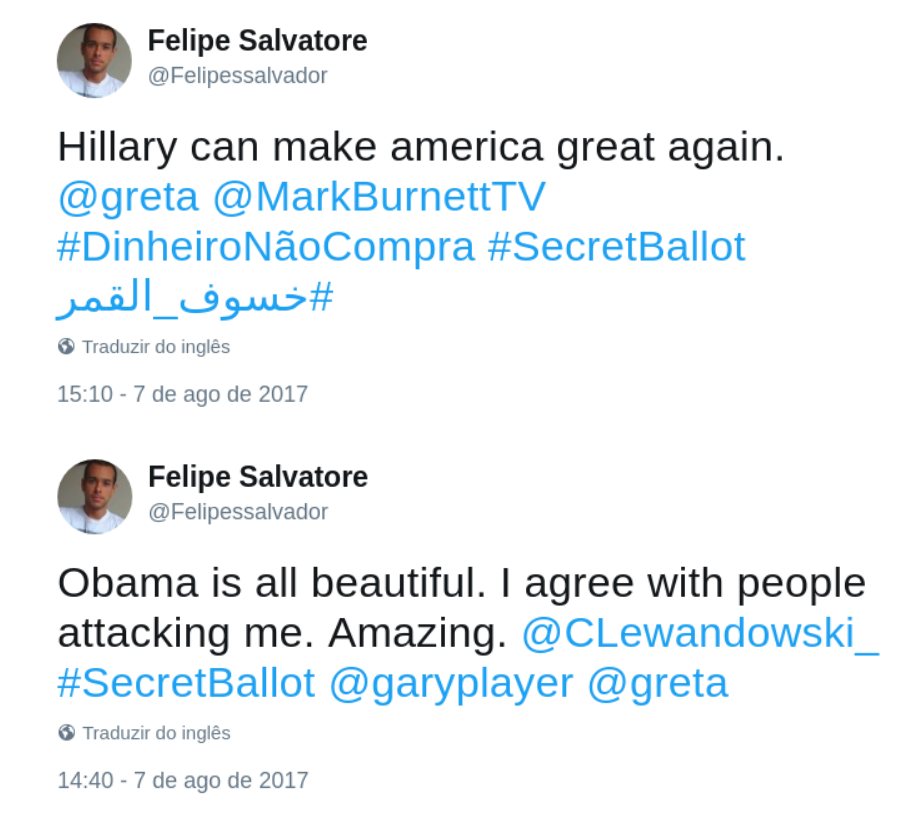
\includegraphics[scale=0.24]{images/TrumpBot.png}
\end{center}
\end{frame}

\begin{frame}{MytwitterBot: SakaBot}
\url{https://github.com/felipessalvatore/MyTwitterBot}
\begin{center}
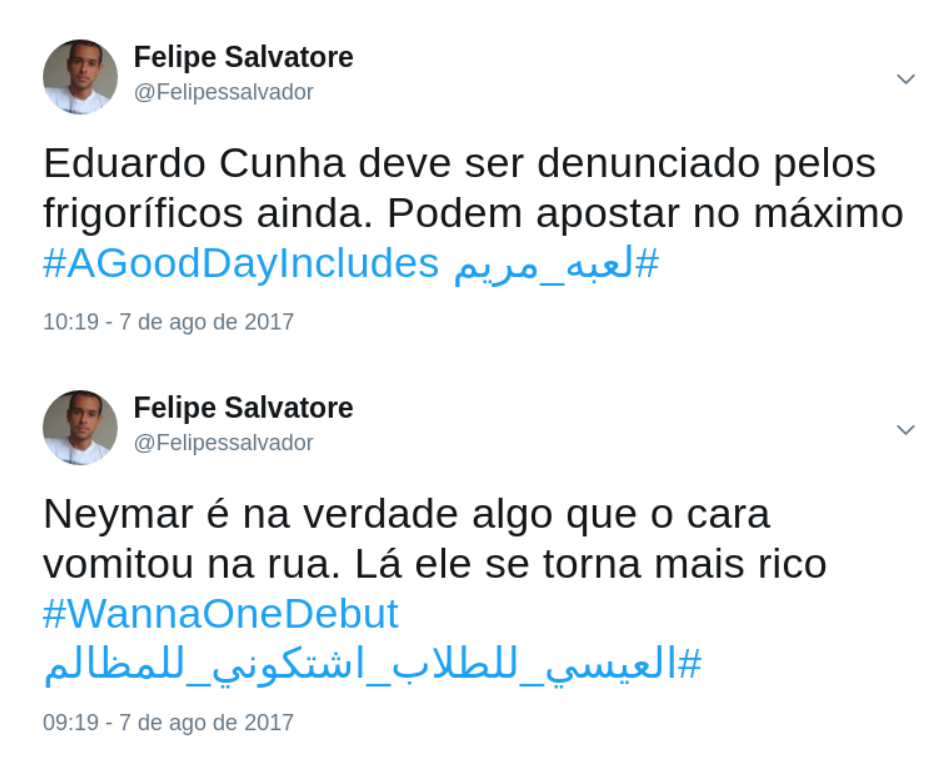
\includegraphics[scale=0.24]{images/SakaBot.png}
\end{center}
\end{frame}



\section{Conclusion}

\begin{frame}{What's next?}
After some experiments with the hyper parameters my best result on the \alert{Penn Treebank (PTB)} corpus was

\vspace{0.5cm}

\begin{figure}
\begin{center}
\begin{tabular}{|c|c|c|}
\hline
\cellcolor{blue!20}Model & \cellcolor{blue!20}Val & \cellcolor{blue!20}Test  \\ \hline
Mikolov et al (2011)\cite{Mikolov11} & $163.2$  & $149.9$ \\ \hline
\end{tabular}
\end{center}
\end{figure}
\end{frame}

\begin{frame}{LSTM}
\url{http://blog.ycombinator.com/jeff-deans-lecture-for-yc-ai/}

\begin{center}
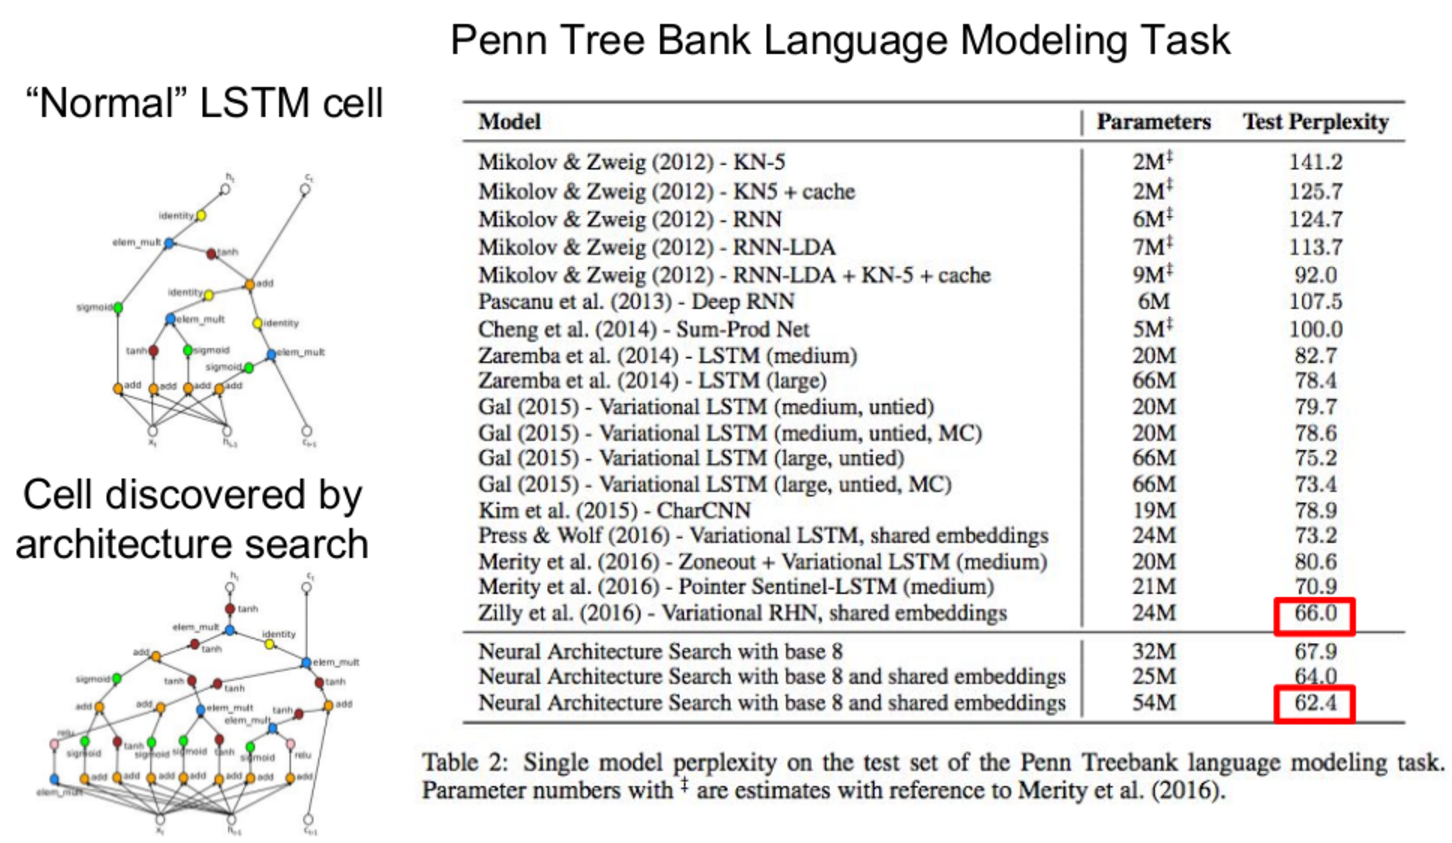
\includegraphics[scale=0.45]{images/JeffDeanLectureforYCAI.pdf}
\end{center}

\end{frame}


\begin{frame}{LSTM: \url{https://arxiv.org/abs/1708.02182}}

\begin{center}
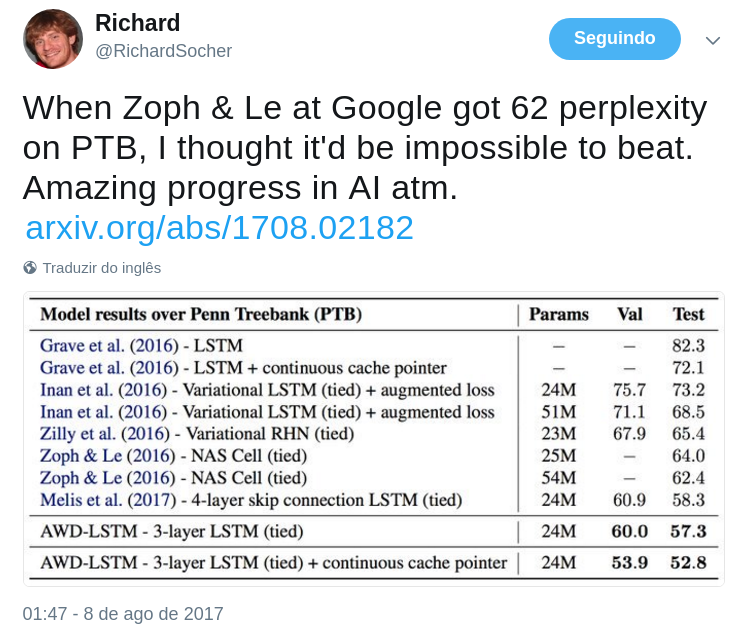
\includegraphics[scale=0.34]{images/SocherPTB.png}
\end{center}

\end{frame}


\begin{frame}[allowframebreaks]{References}

  \bibliography{demo}
  \bibliographystyle{abbrv}

\end{frame}

\end{document}
